\chapter{Configurations and model runs}\label{ch:configurations}

\section{System requirements}
\label{sec:getting-started}

SEAPODYM is a Linux application. When it is used for simulation runs only, namely for simulating population dynamics with fixed (presumably optimal) parameters, there are no specific requirements for the computer configuration. In general, the computer power depends on the numerical model resolutions. For example, Pacific-scale simulations at $1^{\circ}$ spatial resolution and monthly time step can be easily run on a laptop with 8GB of RAM and a 64-bit CPU operating at $2\textrm{GHz}$. However, for higher resolutions and/or global configurations, especially when parameter estimation is envisaged, the advised minimal configuration to run the application efficiently should have a 64-bit CPU at $2\textrm{GHz}$ and higher, with at least $32$~GB of RAM. The physical memory is the key requirement in the case of parameter estimation or other procedures involving the gradient computation. This is because the backward (adjoint) differentiation method stores all intermediate variables needed for the exact evaluation of a cost function gradient in the operational memory. If there is not enough RAM available, the program will dump all temporary data on the hard disk (in files cmpdiff.tmp and gradfil.tmp), which will significantly increase the overall runtime. 

This chapter is for users who want to run the application with the code and executable of the program that are provided. If modifications of some part of the model code are desired, it is highly recommended that the developer's team be contacted, since changes in the code can interfere with computation of the likelihood gradient and hence alter some model functionalities. 
%Read more about memory utilization issues in Chapter ~\ref{ch:optimization}.

\section{Installations}
\label{sec:installations}

Compilation of the source code requires installation of the two additional libraries listed below.

\begin{description}

\item[libxml2] library is used to read and write all application parameters in a text-based {\bfseries xml} parameter file. If it is not installed already, you can download and build the library from 
  \url{ftp://xmlsoft.org/libxml2}

\item[Autodif] libraries provide an array language extension to C ++ enabling the automatic code differentiation \citep{Autodif}. Please visit the \href{www.admb-project.org}{ADMB project} website for the latest release of the \href{http://code.google.com/p/admb-project/downloads/list}{ADModel Builder software}\footnotemark[1] including Autodif libraries and follow the instructions to compile and configure it. 
  
\footnotetext[1]{Note, the program will not use ADModel Builder itself, but only Autodif libraries libado and libadt.}
   
After installation of the ADMB software, you need to declare the environment variable in the .bashrc file pointing to the address where the installed libraries can be found, for example:

\vspace{0.5cm}

{\ttfamily export ADMB\_HOME=/path-to-admb-folder/ }

\vspace{0.5cm}

This variable needs to be specified in the SEAPODYM Makefile. In the case when shared libraries are to be used, add the following in the .bashrc as well:

\vspace{0.5cm}
{\ttfamily export LD\_LIBRARY\_PATH=\$ADMB\_HOME/lib:\$LD\_LIBRARY\_PATH }
\vspace{0.5cm}
 
\end{description}

Once the libraries have been installed and configured, create the source directory, place the code there, edit the provided Makefile.i64 (see Appendix B) to make sure that you have the paths and linker flags recognisable by your gcc compiler, then compile the SEAPODYM application by typing the command:

\vspace{0.5cm}

{\ttfamily make -j -f Makefile.i64} \footnotemark[2]

\vspace{0.5cm}
\footnotetext[2]{The option \texttt{-j} performs a parallel execution of make, and it can be omitted.}

If there are no conflicts in libraries and compiler versions, and all paths are specified correctly, the executable {\bfseries seapodym\_cltags} will be built in the source code directory. It is convenient to create the alias in the .bashrc, for example, {\ttfamily seapodym} to point to this executable, so it can be called without the full path.

\section{Running SEAPODYM with predefined configuration} 
\label{sec:firstrun}

The SEAPODYM-MASS application runs in a command line. Typing the following command:\\

{\ttfamily seapodym -{}-help}\\

provides the usage and the list of available running options:

{\ttfamily 

  Usage: seapodym [options] <parfile name> \\ 

  Options: \\
  \begin{tabular}[here]{lp{9cm}}
    -h, -{}-help 			 & Print this message and exit. \\
    -H, -{}-hessian 		 &Compute Hessian matrix. \\
    -p, -{}-projection 		 &Compute 2D-projection of the likelihood on a grid specified in parfile. \\
    -s, -{}-simulation 		 &Run simulation without optimization. \\
    -sa,-{}-sensitivity-analysis[=FLAG] & Make sensitivity analysis. By default[=0] sensitivity function takes model predictions only. 	If FLAG=1 the sensitivity function takes both predictions and observations.  If FLAG=2 ONE-AT-A-TIME sensitivity analysis. If FLAG=3 ALL-AT-A-TIME sensitivity analysis.  \\
    -t,-{}-twin-experiment[=FLAG], & Perform identical (by default, or FLAG=0) twin experiment. If FLAG=1 the noise will be added to the artificial data. \\
    -v, -{}-version 		 &Print version number and exit. \\
  \end{tabular}
}

\noindent According to this prompt, the program may run with a set of different options, corresponding to available types of runs (described in section~\ref{sec:running-modes}), and requires the configuration file, also called the parfile. However, prior to running the first simulation, one needs to verify the availability of all necessary input data and to configure the paths to these data in the parfile. 

\subsection{Input directories}
\label{sec:inputdir}
First, place the forcing datasets that were provided together with the parfile in the input directories and organise them as shown in Figure~\ref{fig:arborescence_run}. Create two directories, for example, run-OGCMname-domain-resolution and fisheries/spname, for the environmental and the fisheries data respectively. Provide correct absolute paths to these directories in the configuration XML file, in \textcolor{BrickRed}{{\ttfamily strdir}} and \textcolor{BrickRed}{{\ttfamily strdir\_fisheries}}. Second, make sure that the environmental forcing directory contains all necessary input data in binary format and the two ASCII files called mask *.txt and topo*.txt, as shown in Figure~\ref{fig:arborescence_run}. Note also that fisheries data should include spname\_catch\_*.txt file as well as one or several spname\_LF\_*.txt files as described in the XML file (see panels (b) and (c) in Figure \ref{fig:arborescence_run}).

 \begin{figure}[H]
   \centering
    \vbox{
    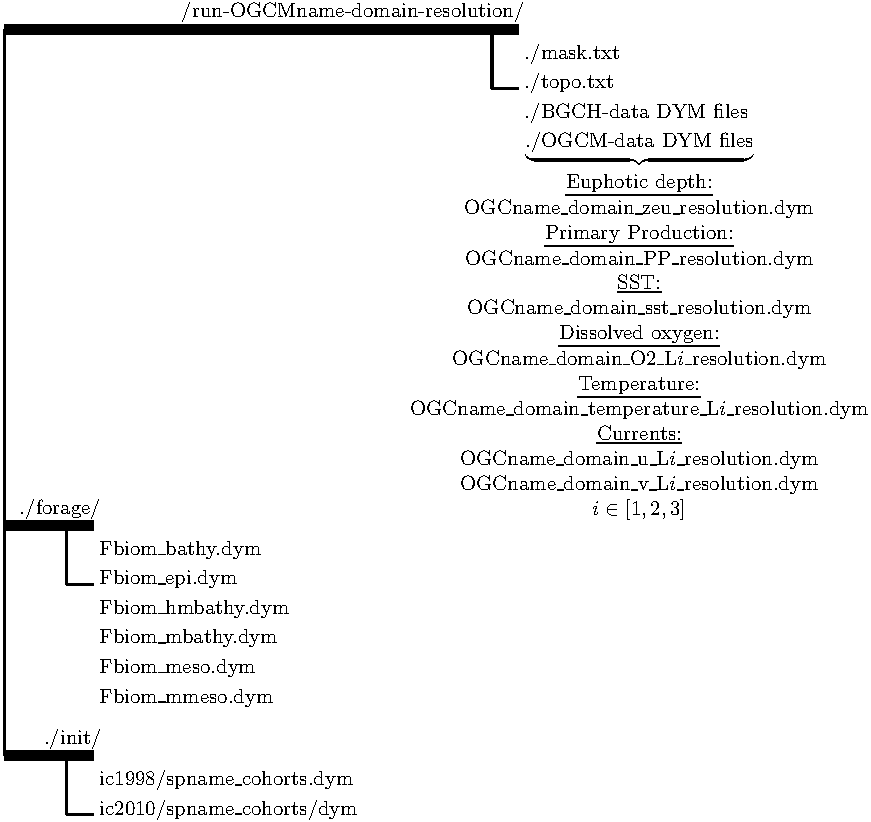
\includegraphics[width=0.7\textwidth]{chapter3/figs/arborescence_run.pdf}\\
    (a)\\
    \vspace{5mm}
    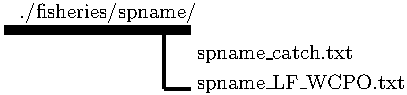
\includegraphics[width=0.4\textwidth]{chapter3/figs/arborescence_fisheries.pdf} \\
   (b) \\
    \vspace{5mm}
   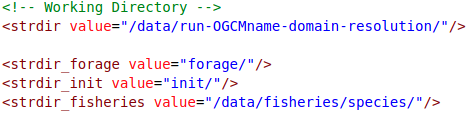
\includegraphics[width=0.6\textwidth]{chapter3/figs/working_input_directory.png} \\
   (c) \\
   }
   \caption{{\bfseries Organising folders and files with SEAPODYM input data.}
   (a) The folder {\ttfamily run-OGCMname-domain-resolution} includes the binary DYM files with environmental data (physical, biochemical and biological forcings) as well as ASCII files with land mask(s) and auxiliary data (topographic index, Exclusive Economical Zones contours), and two subfolders with forage fields and initial conditions. (b) The fisheries data files are stored in a separate folder. (c) Input directories in the configuration file: the paths to the environmental (\textcolor{BrickRed}{{\ttfamily strdir}}) and fisheries data (\textcolor{BrickRed}{{\ttfamily strdir\_fisheries}}) are absolute, whereas the paths to the initial conditions (\textcolor{BrickRed}{{\ttfamily strdir\_init}}) and to the forage data (\textcolor{BrickRed}{{\ttfamily strdir\_forage}}) are relative. }
   \label{fig:arborescence_run}
 \end{figure}

%\noindent In the parfile, both the directories with forcing data (\textcolor{BrickRed}{{\ttfamily strdir}}) and fisheries data (\textcolor{BrickRed}{{\ttfamily strdir\_fisheries}}) are specified as an absolute path. The paths to the files with micronekton data (\textcolor{BrickRed}{{\ttfamily strdir\_forage}}) and to the initial conditions (\textcolor{BrickRed}{{\ttfamily strdir\_init}}), are relative.


\subsection{Simulation run}

When everything is set, you are ready to run the first simulation. It is advisable to create a running directory, where the model will be executed and the output files will be written. The command to run a simulation is: \\

{\ttfamily 
  seapodym -s <parfile name> \\
}

\noindent Note, if the option {\ttfamily -s} is omitted then {\ttfamily seapodym} will actually start minimising the negative log-likelihood according to the configuration in the parameter file {\ttfamily parfile}, and only after completion of the iteration cycle will it run the simulation during which the model output will be written. If this is not desired, for example, if the reference parameter file already contains the MLE solution and the goal is to get the model outputs, then always use the simulation option.

If the first simulation ran successfully, the output folder was auto-generated in the running directory and the output files were written. In this case see section \ref{sec:seapodym-outputs} for a detailed overview of model outputs. Otherwise, if the run ended abnormally, continue reading the following sections to understand the model configuration, to identify and troubleshoot the problem(s).


%\vspace{0.5cm}
%\begin{tabular}{ll}
  % \hline
 % {\ttfamily strdir \textit{value}="absolute-path-to-forcing-data-directory" }& \\
 % {\ttfamily strdir\_fisheries \textit{value}="absolute-path-to-fishing-data-directory" }&  \\
  % \hline
%\end{tabular}

\section{Parameter file}
Configuration of a SEAPODYM run is written in an \texttt{XML} file, called a \textit{parfile} (see full example of a parfile in Appendix~\ref{sec:appendix-parfile}). The following sections explain model configuration through a detailed description of the parfile. \\

\subsection{Spatial domain and resolution}
%\label{subsec:defin-doma-simul}

The model spatial domain is defined by its rectangular geographic area and the complex boundaries within this area. The geographic extension is chosen in line with the knowledge of habitats and migrations of the modelled species: the domain is always set larger than the known area occupied by the population in order to avoid the impact of closed boundary conditions. The complex boundary of the computational domain is described by the land mask (see below). The spatial resolution of the two-dimensional domain is set up by two parameters, {\ttfamily deltaX} and {\ttfamily deltaY}, which define the constant step of the uniform Arakawa-A grid used to resolve model~\ref{eq:model-1} numerically (more details in Chapter~\ref{ch:numerics}). Note that irregularity of the grid is handled in the code through latitudinal correction of the grid cell size. The vertical resolution is accounted implicitly in the model, and is defined by the euphotic depth that is provided as a forcing variable (see below). The number of vertical layers is fixed in the attribute {\ttfamily nb\_layer}. This setup cannot be modified. 

An example configuration for the Pacific Ocean model domain with $2^{\circ}$ resolution is shown in Figure~\ref{fig:domain_space_parfile}. Table~\ref{table:domain_space_parfile} provides a detailed description for each configuration parameter.  

%\begin{adjustbox}{width=1\textwidth}
\begin{table}[H]
\caption{Definition of the domain boundaries and the spatial resolution in the parfile. The names in the left column correspond to the names of the XML nodes.} 
  \begin{tabular}{p{3cm}p{12.5cm}}\hline
    {\bfseries Parameters} & {\bfseries Description}\\ \hline
    \texttt{latitudeMin} & The latitude of the southern grid cell corner, from $+90$N to $-90$S \\
    \texttt{latitudeMax} & The latitude of the northern grid cell corner, from $+90$N to $-90$S \\
    \texttt{longitudeMin} & The longitude of the western grid cell corner, from $0$ to $360$ \\
    \texttt{longitudeMax} & The longitude of the eastern grid cell corner, from $0$ to $360$ \\\hline
    
    \texttt{nb\_layer} & The number of vertical layers  (always~$3$) \\  \hline 
    \texttt{delta\_x} & The grid resolution in longitudinal dimension, in nautical miles \\ 
    \texttt{delta\_y} & The grid resolution in latitudinal dimension, in nautical miles, see eq.~\eqref{eq:delta-xy} and Figure~\ref{fig:Arakawa-A} \\  \hline
    \end{tabular}
\label{table:domain_space_parfile}
\end{table}
%\end{adjustbox}


 \begin{figure}[t]
   \centering
   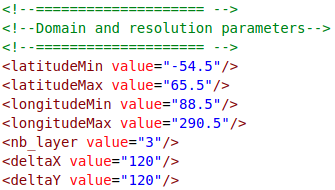
\includegraphics[width=0.4\textwidth]{chapter3/figs/domain_resolution_parameters.png}
   \caption{Example of a computational grid configuration in the parfile. Note that the longitudinal and latitudinal coordinates correspond to the corners of the uppermost grid cells and not the centres of the first and last grid cell.}
   \label{fig:domain_space_parfile}
 \end{figure}

\subsection{Land mask}
\label{sec:land_mask}

The land mask is a matrix with integer values of the size corresponding to the number of grid cells in longitudinal and latitudinal dimensions. The land is denoted ``$0$'' and the ocean cells are defined by non-zero values as follows: $1$ -- only epipelagic layer exists, $2$ -- only two vertical layers exist (i.e., epipelagic and upper mesopelagic), and $3$ -- all three layers exist (epipelagic, upper and lower mesopelagic). The land mask is stored in the ASCII file and its name should be provided in the \textcolor{BrickRed}{{\ttfamily str\_file\_mask}} in the parfile. Note that the mask can be produced and/or modified using the $GMB$ software (see Appendix Toolbox~\ref{appendix-toolbox}). \\

  
\subsection{Time control} 
The time control parameters include the configuration of the time stepping and the simulation time period (Table~\ref{table:time_control}). It is not possible to modify time stepping {\ttfamily iterationNumber} for a given configuration, as it is determined by the temporal resolution of the forcing fields. At the same time, the user can modify the starting and the final date of the run, given that these dates belong to the interval of the forcing data availability. It is advised that the parameter {\ttfamily iterationNumber} is kept unchanged, but higher values can be set to improve the precision of the ADI method. An example of a setup for the time control parameters is shown in Figure~\ref{fig:time_control}. Note that the case of a $30$-day time stepping ($360$-day calendar) is particular, as it corresponds to a virtual $360$-day calendar. In this case the day can be omitted as it is automatically set to $15$.

\begin{comment}
There are a couple of parameters that are not supported any more, such as the number of years for the forecast, {\ttfamily nb\_yr\_forecast}, and the option to activate the model spin-up to generate the initial conditions, {\ttfamily tuna\_spinup}. The forcing data for the forecast time period have to be used as a regular forcing, and the initial conditions can be generated by the separate run, writing the restart file at the end, so both parameters, the {\ttfamily nb\_yr\_forecast} and {\ttfamily tuna\_spinup} can be ignored.
\end{comment}


\begin{table}[H]
\caption{Setting up the temporal resolution of the numerical method and the time range of the simulation.} 
  \centering
  \begin{tabular}{p{3cm}p{12.5cm}}\hline
    {\bfseries Parameters} & {\bfseries Description}\\ \hline
    \texttt{deltaT} & The time step in the outer loop of the numerical model, see $\Delta T$ in (\ref{eq:delta-T}), given in days. It is usually predefined by the time step in the forcing data. \\
    \texttt{iterationNumber} & Number of iterations in the numerical model; it determines the time step in the inner loop of the numerical model, i.e. the time step of the ADI method, see $n_t$ in (\ref{eq:delta-t}). \\  \hline 
     \texttt{save\_first\_date} & Starting date of run, can be any date within the time range of the forcing datasets. The user can specify the year, month and day. \\  \hline 
     \texttt{save\_last\_date} & Final date of run, cannot be earlier than starting date and outside the time range of the forcing datasets. \\\hline 
    \end{tabular}    
\label{table:time_control}    
\end{table}

\begin{figure}[t]
   \centering
   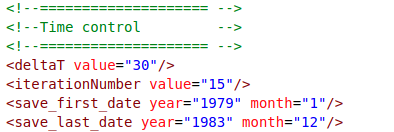
\includegraphics[width=0.5\textwidth]{chapter3/figs/time_control.png}
   \caption{Example of a set-up for the time control parameters.}
   \label{fig:time_control}
 \end{figure}


\subsection{Forcing data}
\label{sec:dym-input}
SEAPODYM relies on multiple oceanic variables to describe the environment of modelled species. These include physical, biochemical and biological forcing variables. Some of them are three-dimensional, such as temperature, dissolved oxygen (O\textsubscript{2}) concentration, zonal/meridional currents and primary production, while others are two-dimensional, such as euphotic depth and functional groups of micronekton. These variables are written in SEAPODYM-specific binary files .dym (Figure~\ref{fig:arborescence_run}) that can be visualised with GUI software called SeapodymView (see Appendix~\ref{appendix-toolbox}). The format of these DYM files is detailed in Appendix~\ref{appendix-DYMfiles}. Note that each file contains the mask and domain information, which should correspond to the model configuration in the XML parfile. 

\subsubsection{Physical and biogeochemical forcing data}
\label{sec:phys-biog-data}
\vspace*{-0.1cm}

The physical forcing dataset includes three physical variables: the temperature (in $^{\circ}$C), and the zonal ($u$) and meridional ($v$) components of the currents (in m$\cdot\text{s}^{-1}$). The biogeochemical fields consist of the primary productivity (in mmol~C$\cdot\text{m}^{-2} \cdot\text{day}^{-1}$), the dissolved oxygen concentration (in ml$\cdot\text{L}^{-1}$), and the euphotic depth (in m).
Prior to being used by SEAPODYM, these forcing variables are always interpolated to a regular Arakawa A grid with the resolution specified by $\Delta X$ and $\Delta Y$ and variable values are placed in the centre of the grid cells. Primary production used in SEAPODYM is vertically integrated throughout the water column (while mostly non-zero in the euphotic zone), whereas the other three-dimensional variables are averaged within the three pelagic layers, defined according to the euphotic depth $Z_{\text{eu}}$ (see Figure~\ref{fig:forcing_integration}). The three vertical layers, $z=(1,2,3)$, are bounded within the intervals $(0, 1.5Z_{\text{eu}})$, $(1.5Z_{\text{eu}}, 4.5Z_{\text{eu}})$, and $(4.5Z_{\text{eu}}, \text{min}(10.5Z_{\text{eu}}, 1000m))$ (see Chapter~\ref{ch:model}, section~\ref{sec:model-forcing} for more details). Therefore, there are nine files with physical oceanographic data, three files with dissolved oxygen data and one for the primary production. \\

In the parfile, besides providing the paths to the directory with forcing data (section~\ref{sec:inputdir} and Figure~\ref{fig:arborescence_run}) and the names of each file (Figure~\ref{fig:physical_biogeochemical_parfile}), the following flags are set up in  {\ttfamily strfile\_oxy} depending on the availability of the oxygen data: $0$ (default) means that the time series of oxygen with the same time step are used in the simulation, $1$ means that the available oxygen data are monthly climatology, and $2$ means that oxygen data have only four spatial fields, each corresponding to one calendar season (January--March, April--June, July--September, October--December).\\

\begin{figure}[t]
   \centering
   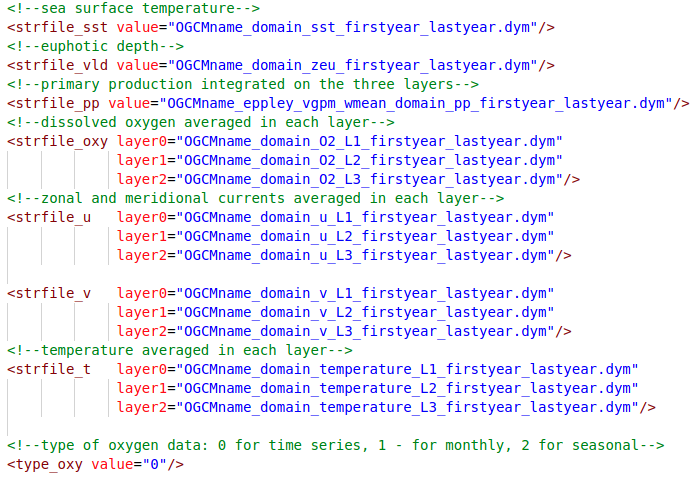
\includegraphics[width=0.75\textwidth]{chapter3/figs/forcing_data.png}
   \caption{The configuration of input forcing variables in the XML parfile using the generic names (the naming convention is not imposed) for physical and biogeochemical forcing data files.}
   \label{fig:physical_biogeochemical_parfile}
 \end{figure}

Note that contrary to the previous SEAPODYM-MASS versions, the monthly climatology variables are no longer used in the model. For technical reasons these variables, as well as their file names, are kept in the code and can be present in the parfile; however, the program does not require these files. 

\subsubsection{Mid-trophic level biomass}
\label{sec:mtl}

The biological forcing of SEAPODYM-MASS consists of six functional groups of micronekton, representing the prey fields of modelled species. The modelling of the mid-trophic functional groups (i.e. micronekton) is done separately by the SEAPODYM-LMTL submodel based on the same forcing fields of temperature, currents and primary production. The six files produced by SEAPODYM-LMTL, one per functional group, contain the potential biomass (in $\text{gWW}\cdot\text{m}^{-2}$) of micronektonic organisms as shown in Figure~\ref{fig:mnk_groups}. These variables are also written in DYM format. The names of these files are composed from prefix {\ttfamily Fbiom} and the names of the micronekton functional groups that are listed under the {\ttfamily frg\_name} tag in the parfile (see section~\ref{sec:prey_model}). Note that a non-conformance of these names in the forcing directory and the parfile will lead to the runtime error.  


\subsubsection{Initial conditions} 
\label{sec:init-dym}
Initial condition, that is, the model state vector at time $t_0$, $N(a,t_0,x,y)$ in (eq.~\ref{eq:model-1}), is the solution of the numerical model obtained for the date preceding the beginning of the run by one time step. The file with initial conditions, also called the  \textit{restart} file (see also section~\ref{restart-dym}) is automatically generated at the end of each simulation and written in the output directory. The structure of this file, written in the DYM format, is a series of two-dimensional density fields for all age classes from $a_0$ to $A+$ at time $t_0$. Thus the third dimension, {\ttfamily Zlevel} (see Appendix~\ref{appendix-DYMfiles}), in this file is age and not time. The name of this file is spname\_cohorts.dym, where the species short name {\ttfamily spname} is declared in the parfile under the {\ttfamily sp\_name} tag. In order to be taken into account by the seapodym application, the initial condition file should be placed into a subfolder called {\ttfamily init}, and its relative path should be declared in the {\ttfamily strdir\_init} attribute of the parfile (panel (c), Figure~\ref{fig:arborescence_run}).  


\subsubsection{Fisheries data}
\label{sec:fishing-data}
The anthropogenic forcing is represented by fisheries data, that is, effort-and-catch and length frequencies. These variables are written in ASCII format (see Appendix~\ref{appendix-ascii}) in a tabular format and not as the two-dimensional fields. This is because the effort and catch data are usually sparse data. The path to the directory with fishing data (see Figure~\ref{fig:arborescence_run}) is specified in \textcolor{BrickRed}{{\ttfamily strdir\_fisheries}} in the parfile. As there are two types of fisheries data, there are two types of files -- one file, spname\_catch\_*.txt, containing the effort and catch (EC) data and one or more files, spname\_LF\_*.txt, with length frequency (LF) data (see Figure~\ref{fig:catch_effort_data}). The formats of these files are detailed in Appendix~\ref{appendix-ascii}. Note, if LF data are stored in multiple files (e.g., coming from different sources with distinct regional structure), the LF data files must be listed in the parfile in the sequential order of the sampling regions found in the file headers (Appendix~\ref{appendix-ascii}), as file1, file2 etc. (Figure~\ref{fig:catch_effort_data}). 

The temporal resolution of EC data should be the same as the resolution of the model, that is, $\delta T$. The spatial resolution of EC data can be different, but unique within a single fishery (see declaration of fisheries in section~\ref{sec:config-fisheries}). The model application can handle coarser spatial resolutions of EC data. In the case when it is finer than the model spatial resolution, the data will be simply summed up within the model grid cell. Currently, the numerical model accepts only the quarterly and regional LF data. 

\begin{figure}[t]
   \centering
   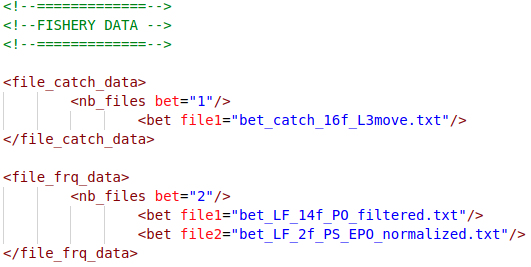
\includegraphics[width=0.6\textwidth]{chapter3/figs/catch_effort_data.png}
   \caption{Catch and effort data files in the parfile.}
   \label{fig:catch_effort_data}
 \end{figure}

\subsubsection{Topographic index}
One more type of input data can be used by SEAPODYM to limit the movement of fish towards coastal areas with shallow topography. The topographic index is the matrix with real values between 0 and 1, which act as multipliers to the habitat index that drives movement of young and mature adult age classes (see classification in Table~\ref{tab:life_stages}). The small values of this index indicate the less accessible (shallow) areas, and values ``1'' indicate no effect of topography on the habitat and hence movement. The use of topographic index is optional. In the case when the topography is not considered, the file does not need to be specified in the parfile. Current reference configurations may include the topographic index generated with the help of the algorithm in the GMB software.


 \begin{figure}[t]
   \centering
    \vbox{
    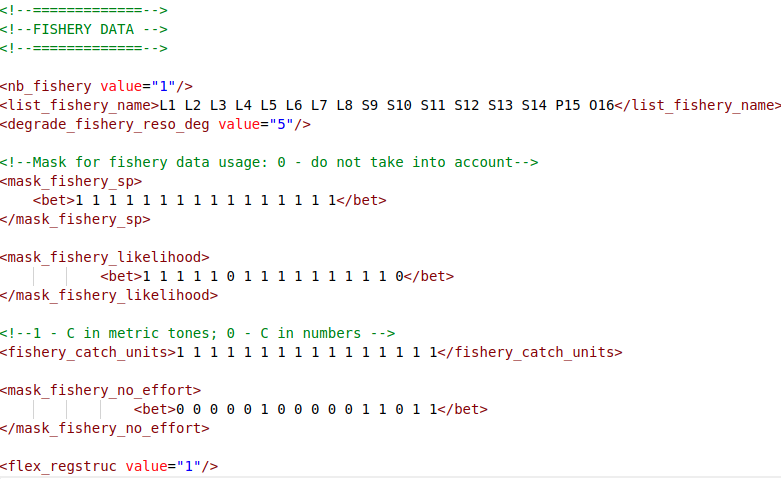
\includegraphics[width=0.9\textwidth]{chapter3/figs/fishery_data_1.png}}
   \caption{Example of the fisheries configuration in the parfile. }
    \label{fig:fisheries_parfile}
 \end{figure}

\subsection{Fisheries configuration} \label{sec:config-fisheries}

There are multiple configuration parameters related to the use of fisheries data in simulations (Table \ref{tab:configuration_fishery}). They specify the number of fisheries, their short names, the units of catch, the flags controlling the use of fisheries as the model forcing (fishing mortality), the flag for catch prediction method, the resolution and the use of each fishery in the likelihood (see example in Figure~\ref{fig:fisheries_parfile}). The fishery short name, or fishery ID, is constructed from the letter corresponding to the gear code and the fishery index in file spname\_catch*.txt. For example, the fishery short name {\ttfamily L1} refers to the first fishery in the dataset being the long-line fishery. 

Note that the effort and catch data provided on coarser spatial resolutions will be redistributed to the resolution of the model to compute fishing mortality, but used at the original or even coarser resolution in the catch prediction method. In other words, the predicted catch will either be at the spatial resolution at which the original data were collected, or, if the option {\ttfamily degrade\_fishery\_reso\_deg} is set to a resolution coarser than the original fisheries resolution and that of the model, then the resolution of the predicted catch of all eligible fisheries will be degraded to a specified value. The information about initial and final spatial resolutions of all fisheries will be printed in the screen log of the simulation. \\

\begin{table}[H]
\caption{Fisheries configuration parameters. The names in the left column correspond to the names in the XML parameter file.}
  \begin{tabular}{p{5.2cm}p{10.5cm}}
    \hline
    {\bfseries Parameters} & {\bfseries Description}\\ \hline\hline
    {\ttfamily nb\_fishery}  & Number of fisheries, $n_{f}$, in the current configuration.\\\hline
    {\ttfamily list\_fishery\_name} & List of fishery short names of length $n_f$. These fisheries must be present in file spname\_catch*.txt. \\\hline
    {\ttfamily degrade}\_{\ttfamily fishery}\_{\ttfamily reso}\_{\ttfamily deg} & Resolution (in degrees) to degrade fisheries data in the model predictions only.\\\hline
    {\ttfamily mask\_fishery\_sp}  & A vector of integers of length $n_f$ to activate (1) or deactivate (0) fisheries in the model run. \\\hline
    {\ttfamily mask}\_{\ttfamily fishery}\_{\ttfamily likelihood} & Same as above, but influences the likelihood computation only. It means that if the fishery is active in ``mask\_fishery\_spname'', but turned off in this flag, it still causes fishing mortality, but predicted catch and/or LF of this fishery are not accounted in the likelihood. \\\hline
    {\ttfamily fishery\_catch\_units} & A vector of integers of length $n_f$ to specify the units of the observed catch in the fishery: 1 for metric tonnes, 0 for numbers. \\\hline
    {\ttfamily mask\_fishery\_no\_effort}  & A vector of integers of length $n_f$ to specify which fishery do not have effort data: 0 if the fishery has effort data, 1 if fishery does not have effort data. The catch removal method is used for fisheries without effort. \\\hline
\end{tabular}
\label{tab:configuration_fishery}
\end{table}

\subsection{Likelihood function configuration} \label{sec:config-likelihood}

Regardless of the type of the run (see section~\ref{sec:running-modes}), the likelihood function specified in the parfile will be computed and the current (cumulative) value will be displayed at every time step and at the end of the simulation. The negative log-likelihoods are computed and reported by data type in the following order: catch likelihood, length frequency likelihood, tagging data likelihood and the average stock function. Since this chapter is devoted to a simulation run with a predefined configuration, this section aims to provide only the short description of likelihood parameters, configured through the parfile (Table~\ref{tab:configuration_likelihood}). For their meaning and respective function, please read Chapter~\ref{ch:parametrisation}.

\begin{table}[H]
\caption{Likelihood configuration parameters. The names in the left column correspond to the names in the XML parameter file.}
\begin{tabular}{p{4.5cm}p{11.2cm}}
    \hline
    {\bfseries Parameters} & {\bfseries Description}\\ \hline\hline
    {\ttfamily nb\_step\_to\_skip} & A number of model time steps to skip before starting augmenting the likelihood. It is advisable to skip at least one age at maturity of the modelled species in order to give the model a time to renew the population biomass based on current parameters. \\\hline
    {\ttfamily total\_likelihood} & The total likelihood value corresponding to current configuration. Note, this value will be written in the {\ttfamily newparfile.xml} created upon finishing the model run, and not in the parfile that was provided at execution. \\\hline
    {\ttfamily like\_c\_cpue} & The flag for using catch or CPUE (catch per unit effort) data in the likelihood: if ``$0$'' the catch is used in the likelihood, if ``$1$'' the CPUE.\\\hline
    {\ttfamily likelihood\_types}& A vector of integers of length $n_f$ (Table~\ref{tab:configuration_fishery}) for likelihood type selection for each fishery: concentrated (1), log-normal (2), Poisson (3), negative binomial (4), zero-inflated negative binomial (5), truncated Poisson (6). \\ \hline
    {\ttfamily frq\_likelihood} & A flag to include (1) or exclude (0) the length frequency term from the likelihood. \\ \hline
    {\ttfamily tag\_likelihood} & A flag to include (1) or exclude (0) the tagging data term from the likelihood. \\ \hline
    {\ttfamily tag\_likelihood\_only} & A simulation type flag. If this flag is set to ``1'', then only the movement model of tagged tuna sub-population density will be numerically resolved. Use this flag only for tag simulator or estimation of movement parameters from tagging data (see Chapter~\ref{ch:parametrisation}).\\ \hline
    {\ttfamily stock\_likelihood} & A flag to add the average stock constraint into the likelihood ($\beta$ in eq.~\ref{eq:beta-like}): ``$1$'' to include, ``$0$'' otherwise. \\ \hline 
    {\ttfamily mean\_stock\_obs} & The average biomass ($\overline{B}$ in eq.~\ref{eq:beta-like}) over the rectangular region specified within this attribute. It is used only if {\ttfamily stock\_likelihood} is activated. \\ \hline
    {\ttfamily likelihood\_parameters} & A set of negative binomial dispersion parameters, ($\beta_f$ in eq.~\ref{eq:negbin}), one per fishery. These parameters are effective (and can be estimated) only if the {\ttfamily likelihood\_types} are set to 4 or 5 for corresponding fisheries. \\ \hline 
    %Therefore, it might have up to $n_f$ standard deviation to set configure. 
    {\ttfamily prob\_zero} & A set of negative binomial probability of null observation parameters ($p_f$ in eq.~\ref{eq:negbin}), one per fishery. These parameters are effective (and can be estimated) only if the {\ttfamily likelihood\_types} are set to 4 or 5 for corresponding fisheries. \\ \hline
    \hline
\end{tabular}
\label{tab:configuration_likelihood}
\end{table}

% \begin{figure}
%   \centering
%    \vbox{
%    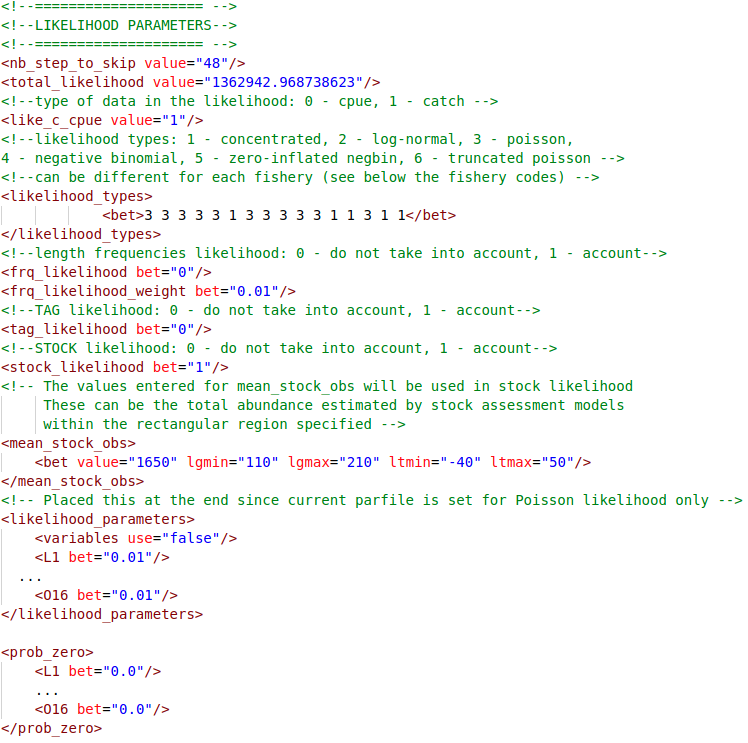
\includegraphics[width=0.9\textwidth]{chapter3/figs/likelihood.png}\\
%   }
%   \caption{{\bfseries} Example of likelihood configuration parameters in the parfile.} 
%   \label{fig:likelihood_parfile}
% \end{figure}

\subsection{Dynamic model parameters}

\subsubsection{Prey model parameters}
\label{sec:prey_model}
Some SEAPODYM-LMTL model \citep{Lehodey1998, Lehodey2010, Lehodey2015} parameters are used in the SEAPODYM-MASS model. Besides, SEAPODYM-MASS is designed to run in predator--prey mode, thus coupling predator and prey dynamic models. However, since all existing reference models are based on offline coupling, and the fully coupled model is not regularly maintained in the software, we do not discuss it here. Table~\ref{tab:conf_prey_model}  details all configuration parameters for micronekton. Note that those SEAPODYM-LMTL parameters that do not affect SEAPODYM-MASS solution are listed in the parfile only for information purposes.  

\begin{table}[H]
\caption{The micronekton configuration parameters in the parfile. Note that SEAPODYM-LMTL parameters marked with ``*'' are effective only in the predator--prey coupling mode.}
\begin{tabular}{p{3.5cm}p{12.0cm}}
    \hline
    {\bfseries Parameters} & {\bfseries Description}\\ \hline\hline
    {\ttfamily Tr\_max}$^*$ & The maximal time before recruitment to micronekton. \\\hline
    {\ttfamily Tr\_exp}$^*$ & The slope of temperature-dependent function of recruitment time. \\\hline
    {\ttfamily inv\_lambda\_max}$^*$ &  The inverse of maximal mortality rate. \\\hline
    {\ttfamily inv\_lambda\_curv}$^*$ &  The slope of temperature-dependent mortality function. \\\hline
    {\ttfamily c\_pp} & Conversion constant from primary production to wet weight of mikronekton. \\\hline
    {\ttfamily E} & Energy transfer coefficient from primary production to trophic level of micronekton. \\\hline
    {\ttfamily nb\_forage} & Number of functional groups. Refers to the number of non-zero elements in matrix $F$ (eq.~\ref{eq:F}).\\\hline
    {\ttfamily source\_frg}$^*$ & The coefficients of repartition of energy transfer among functional groups of micronekton.  The sum of six coefficients should always give $1$. \\\hline
    {\ttfamily frg\_name} & The names of the functional groups of preys (see Table~\ref{tab:forage-in-layers}). \\\hline
    {\ttfamily day\_layer } & The index of the daytime vertical layer (0,1,2) of functional group (see Figure~\ref{fig:mnk_groups}). \\\hline
    {\ttfamily night\_layer} &  The index of the night-time vertical layer (0,1,2) of functional group (see Figure~\ref{fig:mnk_groups}). \\\hline
    {\ttfamily sigma\_fcte} & Diffusion rate (nmi$^2\cdot$day$^{-1}$).\\ \hline
\end{tabular}
\label{tab:conf_prey_model}
\end{table}

% \begin{figure}[t]
%   \centering
%    \vbox{
%    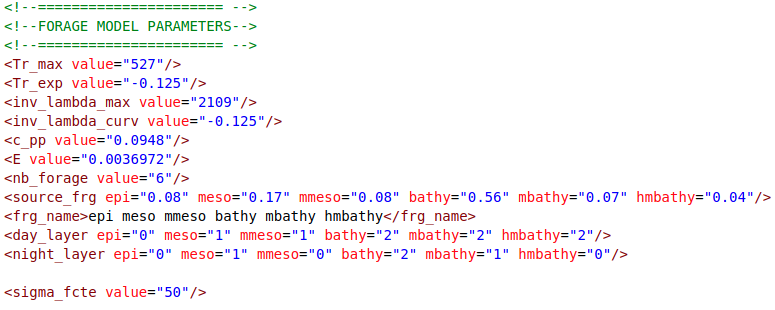
\includegraphics[width=1.1\textwidth]{chapter3/figs/new_print_forage_model.png}
%   }
%   \caption{Forage model parameters in the parfile.}
%   \label{fig:forage_parfile}
% \end{figure}

All six functional groups of micronekton defined in the SEAPODYM-LMTL model should be declared in the parfile. Attention should be paid to the forage names ({\ttfamily frg\_name}). First, as pointed out earlier, these names are used in the input files with micronekton densities (section~\ref{sec:mtl} and Figure~\ref{fig:arborescence_run}). Second, they provide the names of model parameters $E_{ij}$ (eq.~\ref{eq:eF-matrix}) in the parfile, see Table~\ref{tab:habitats-xml}. It is advisable not to modify these names to ensure stability of the model software. The correspondence between forage names and model notations for the micronekton functional groups is shown in Table~\ref{tab:forage-names}.   

\begin{table}[H]
\captionof{table}{The forage names, the model notations and vertical layer set-up in the parfile.} 
\begin{center}
\begin{tabular}{c}
  \begin{tabular}{|p{3.5cm}||>
  {\centering}p{1.6cm}|>
  {\centering}p{1.6cm}|>
  {\centering}p{1.6cm}|>
  {\centering}p{1.6cm}|>
  {\centering}p{1.6cm}|>
  {\centering\arraybackslash}p{1.65cm}|}

    \hline
    {\ttfamily \textbf{frg\_name}} & {\ttfamily \textbf{epi}} & {\ttfamily \textbf{meso}} & {\ttfamily \textbf{mmeso}} & {\ttfamily \textbf{bathy}} & {\ttfamily \textbf{mbathy}} & {\ttfamily \textbf{hmbathy}} \\
    \hline
    \textbf{model notation} & $F_{11}$ & $F_{22}$ & $F_{21}$ & $F_{33}$ & $F_{32}$ & $F_{31}$ \\
    \hline
    {\ttfamily \textbf{day\_layer}} & 0 & 1 & 1 & 2 & 2 & 2 \\
    \hline
     {\ttfamily \textbf{night\_layer}} & 0 & 1 & 0 & 2 & 1 & 0 \\
    \hline
  \end{tabular}\\
\end{tabular}
\label{tab:forage-names}
\end{center}
\end{table}

The following micronekton parameters (Table~\ref{tab:conf_prey_model}) affect the numerical solution of the SEAPODYM-MASS model. The pair {\ttfamily c\_pp} and {\ttfamily E} are used to compute the wet weight of plankton ($\Lambda$ in eq.~\ref{eq:spawning-prey}). The diffusion of larvae and small juveniles, which are assumed to have similar properties to the micronekton organisms, is governed by diffusion rate {\ttfamily sigma\_fcte} defined in the  micronekton model to account for small-scale movements of fish and diffusion of water masses. Most important is the definition of the vertical structure of the micronekton functional groups, described in the attributes named {\ttfamily day\_layer} and {\ttfamily night\_layer} (Table~\ref{tab:forage-names}). These parameters are essential, as they determine key dynamic processes of the SEAPODYM model, such as movements (via accessibility of predators to prey, habitats and movement rates) and larval survival. The set-up of these vectors yields the day and night structure shown in Table~\ref{tab:forage-in-layers}).  \\

\begin{table}[H]
\captionof{table}{Total biomass density of functional groups of micronekton present during the day/night in each vertical layer are sums of the rows/columns in matrix $\mathbf{F}$ (eq.~\ref{eq:F}). } 
\begin{center}
\begin{tabular}{c}
  \begin{tabular}{|c||c||c|}

    \hline
    \textbf{layer name}& \textbf{day} & \textbf{night} \\
    \hline
    \hline
    epipelagic   & $F_{11}$  & $F_{31}+F_{21}+F_{11}$ \\
    \hline
    upper mesopelagic & $F_{21}+F_{22}$ &  $F_{32}+F_{22}$  \\
    \hline
    lower mesopelagic & $F_{31}+F_{32}+F_{33}$  & $F_{33}$\\
    \hline
  \end{tabular}\\
\end{tabular}
\label{tab:forage-in-layers}
\end{center}
\end{table}

\subsubsection{Predator model parameters}\label{sec:species_model}
The current version of the model software supports only a single-species model, so the value of the XML tag {\ttfamily nb\_species} should always be set to 1. The species short name, {\ttfamily spname}, usually corresponds to the species code of the \href{http://www.fao.org/fishery/statistics/tuna-catches/en}{\textbf{FAO}} convention. Note, the species short name provided in {\ttfamily nb\_species} is used throughout the parfile as well as in various model outputs (file names, headers etc., see section~\ref{sec:seapodym-outputs}). For example, the short name ``bet'' is used for bigeye tuna (Figure~\ref{fig:age_structure_parfile}), and all XML attributes describing species parameters, either related to its fisheries, to the likelihoods or to the model, have this short name.\footnote{Note, in the case of a short name modification, simply replace all occurrences in the XML file with the new name.} Bigeye model parameters then appear with the following formatting:

\begin{center}
{\ttfamily <parameter\_name bet="value"/> \\}
\end{center}

\noindent See other examples in Figure~\ref{fig:age_structure_parfile} and the parfile in Appendix~\ref{sec:appendix-parfile}. 

\begin{figure}[t]
   \centering
    \vbox{
    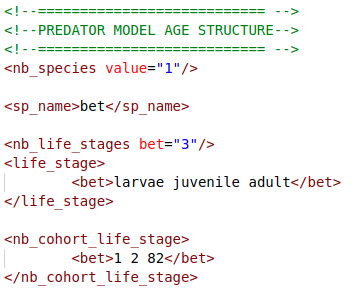
\includegraphics[width=0.45\textwidth]{chapter3/figs/new_print_age_structure}\\
   }
   \caption{{\bfseries} The example of the species declaration and configuration of the life stage structure for bigeye tuna in the parfile.}
   \label{fig:age_structure_parfile}
 \end{figure}

\subsubsection{Age and life stage parameters} 
Age and life stage parameters are essential configuration parameters that describe the species' age and life stage structure as well as its main biological characteristics -- maturity, length and weight at age (Table~\ref{tab:model_age_structure}). All these parameters are used as predefined constants in the model, meaning that they do not vary in time and space and currently cannot be estimated. However, since the age structure plays an important role in the definition of habitats, movement rates, recruitment, mortality and predicted fisheries statistics (eqs.~\ref{eq:Nmature}, \ref{eq:temperature-length}, \ref{eq:sigma-weight}, \ref{eq:M}, \ref{eq:catch-in-weight}), modification of these parameters can alter model outputs and provide the model state, which does not correspond to the MLE solution. Therefore it is advisable not to modify these parameters in the reference configuration without subsequent parameter estimation (see Chapter~\ref{ch:parametrisation}).

\begin{table}[H]
\caption{Configuration of the species life stages, age structure, growth and maturity parameters.}
\begin{tabular}{p{4.25cm}p{11.25cm}}
    \hline
    {\bfseries Parameters} & {\bfseries Description}\\ \hline\hline
    {\ttfamily nb\_life\_stages} & The number of the species life stages to be considered in the model (see Table~\ref{tab:life_stages} for more details). \\
    {\ttfamily life\_stage} & List of names of the life stages (Figure~\ref{fig:age_structure_parfile}). \\
    {\ttfamily nb\_cohort\_life\_stage} &  A vector of size {\ttfamily nb\_life\_stages} giving the number of age classes by life stage.  \\\hline
    {\ttfamily sp\_unit\_cohort} & A vector of $\Delta a$ (the size of age class in days) of length $n_a=\sum{\texttt{nb\_cohorts\_life\_stage}}$. \\\hline
    {\ttfamily age\_recruit} & Age at recruitment to the exploited stock. It is used solely for comparison with stock assessment models.\\    
    {\ttfamily age\_mature} & The age at first maturity (50\% maturity). This parameter is ignored if values of maturity-at-age are provided explicitly for all age classes. \\
    {\ttfamily maturity\_age} & The vector of maturity-at-age estimates ($\mu(a)$ in eq.~\ref{eq:Nmature}) of length $n_a$. The values between 0 and 1 give the proportion of mature adults in each age class. \\\hline    
    {\ttfamily length} & A vector of mean fork lengths of fish ($\ell(a)$ in eq.~\ref{eq:vonBertalanffy}, in cm) of length $n_{a}$, estimated in the middle of each age class. \\
    {\ttfamily weight} & A vector of mean weights of fish ($w_a$ in eq.~\ref{eq:weight-at-length}, in kg) of length $n_{a}$, estimated in the middle of each age class.\\
    \hline
\end{tabular}
\label{tab:model_age_structure}
\end{table}

There are a few rules to know with respect to age structure definitions in SEAPODYM. First, the number of age classes in the larvae cohorts is always 1, whatever the size of the age classes, $\Delta a$. Second, all age classes but the last one, $A+$, have the same size. It is best to have $\Delta a = \Delta T$; however, the software can manage the cases when $\Delta a > \Delta T$, if $\Delta a$ is divisible by $\Delta T$. Note that in the latter case, the ageing dynamics will be computed every $\frac{\Delta a}{\Delta T}$ time steps (see section~\ref{sec:age-integration} in Chapter~\ref{ch:numerics}); hence the model's numerical solution can be considered valid only at the end of $\Delta a$ intervals. Third, the young (immature adult) life stage does not need to be specified in {\ttfamily life\_stage} and {\ttfamily nb\_cohort\_life\_stage} as it is defined automatically by the maturity vector {\ttfamily maturity\_age} or the age at first maturity {\ttfamily age\_mature}. 

Note, the section devoted to the description of the species age structure may contain one more vector, called {\ttfamily age\_compute\_habitat}, which is not related to the definition of the species age structure, but can be specified to shorten the runtime of the simulation by avoiding re-computing habitat values (and hence velocities) until significant change in mean length occurs between age classes. This can be especially useful in the optimization runs (see section~\ref{sec:fmin}). 

\subsubsection{MLE parameters}
\label{sec:mle_parameters}

This section describes parameters that can be estimated via the Maximum Likelihood Estimation method. All the dynamic model parameters that can be set as control parameters in optimization have the following format:\\ 

\noindent
{\ttfamily 
\makebox[1.5cm]{} <parameter spname = "value"> \\
\makebox[1.5cm]{} <variable min="minimal\_value" max="maximal\_value" use="true"/> \\
\makebox[1.5cm]{} </parameter>\\
} 

\noindent where the ``value'' is the current parameter value in the model, and the minimal and maximal values are the boundaries within which the parameter is allowed to vary in optimization. The attribute {\ttfamily use="true"} activates the use of a given parameter as a control variable in optimization. Any other word put in the attribute ``use'' removes the parameter from the list of control variables. Note that boundary values are designed for the optimization runs, but they can affect the parameter value in the simulation run as well if (and only if) the attribute {\ttfamily use="true"} and the value of a given model parameter lies outside its boundaries. In this case the software automatically resets the parameter to a value close to the nearest boundary.

Tables~\ref{tab:demography-xml}--\ref{tab:fisheries-xml} summarise model parameters that can be estimated. These tables are extensions of Table~\ref{tab:parameters} with SEAPODYM dynamic model parameters, providing also the parfile names\footnotemark[1] in order to show their correspondence with the mathematical notations in model~\ref{eq:model-1}, and linking their set-up (when necessary) with other configuration parameters in the XML file.

\footnotetext[1]{Note also, that the names in the parfile are the same as in the SEAPODYM computer code.}

\begin{table}[H]
\caption{Species demographic parameters with their notations in the parfile and in model~\ref{eq:model-1}, definitions and references.}
  \begin{tabular}{p{3.6cm}p{1.5cm}p{10.25cm}}\hline
   \textbf{Parfile name} & $\boldsymbol \uptheta$	(\textbf{Eq.}) & \textbf{Description}	\\\hline 
     \multicolumn{3}{c}{\textit{Recruitment}} \\
    \hline
    \texttt{nb\_recruitment} & $r$~\eqref{eq:larvae} & {Reproduction rate in Beverton--Holt function, in $\text{mo}^{-1}$.}\\
    \texttt{a\_adult\_spawning} & $b$~\eqref{eq:larvae} & {Slope parameter in Beverton--Holt function, in $\text{Nb}/\text{km}^2$.}\\\hline
     \multicolumn{3}{c}{\textit{Natural mortality}}\\
    \hline
    \texttt{Mp\_mean\_max}& $\bar{m}_p$~\eqref{eq:Mp} & {Predation mortality rate at age $0$, in $\text{mo}^{-1}$.}\\

    \texttt{Mp\_mean\_exp}& $\beta_p$~\eqref{eq:Mp} & {Slope coefficient in predation mortality.} \\

    \texttt{Ms\_mean\_max}& $\bar{m}_s$~\eqref{eq:Ms} & {Senescence mortality rate at age $0$, in $\text{mo}^{-1-\beta_s}$.}\\

    \texttt{Ms\_mean\_slope} & $\beta_s$~\eqref{eq:Ms}  & Slope coefficient in senescence mortality.\\

    \texttt{M\_mean\_range} & $\epsilon$~\eqref{eq:Mvar} & {Variability of mortality rate with habitat index from $\frac{M}{(1+\epsilon)}$ in the worst habitat to $M(1+\epsilon))$ in the best habitat.} \\\hline
%\multicolumn{3}{c}{\texttt{Food requirement index}}\\
%    \hline
%    $R$ &\texttt{forage\_ration}& {Daily food ration. This parameter is also used to compute predation mortality that is activated in predator-prey coupled model.}\\
%
%    $r_c$  &\texttt{residual\_competition}& {Residual competition is the proportion of total F biomass available for a given species in the presence of other species.} \\
%    \hline		    
  \end{tabular}
\label{tab:demography-xml}  
\end{table}

Table~\ref{tab:demography-xml} includes demographic, that is, reproduction and mortality parameters. Note that there are other model parameters that affect the population size and age composition, such as spawning habitat (see eq.~\ref{eq:larvae}) and fisheries parameters (eq.~\ref{eq:FM}), but compared to demographic parameters, the latter have spatial effects and/or additional functions. For example, spawning habitat parameters can modify the total number of larvae recruited as well as overall population spatial distribution. Fisheries parameters affecting the total population mortality also control the model predictions, catch and length frequency. 

Table~\ref{tab:habitats-xml} describes all habitat-related parameters, for both spawning and feeding habitats (see sections~\ref{sec:spawning-habitat} and \ref{sec:feeding-habitat}). There exist two alternatives for the use of spawning habitat parameters. First, all habitat parameters can be used independently exactly as presented in Table~\ref{tab:habitats-xml}. Second, the assumption that the species' preferred range and the target temperature are the same as the range and the temperature that are optimal for larval survival (see Chapter~\ref{ch:model}, section~\ref{sec:age-dependence}), can be set up via the XML parameter {\ttfamily uncouple\_sst\_larvae spname="0"} (see also section~\ref{sec:model-options} below). Thus, assuming that $\sigma_0=\sigma$ and $T_0=T^*$, this set-up reduces the number of model parameters. In this case, parameters {\ttfamily a\_sst\_larvae} and {\ttfamily b\_sst\_larvae} are ignored and {\ttfamily a\_sst\_spawning} and {\ttfamily b\_sst\_spawning} are used in the equation of spawning habitat index (eq.~\ref{eq:spawning-thermal}) and in the age-dependence of predators' thermal accessibility to prey organisms (eqs.~\ref{eq:temperature-length} and \ref{eq:sigma-weight}).


\begin{longtable}{p{3.75cm}p{1.75cm}p{9.75cm}}
\caption{Habitat parameters with their notations in the parfile and in model~\ref{eq:model-1}, definitions and references.\label{tab:habitats-xml}}\\\hline
\textbf{Parfile name}	& $\boldsymbol \uptheta$ (\textbf{Eq.})&  \textbf{Description} \\\hline 
\endfirsthead
%\multicolumn{3}{@{}l}{\ldots continued}\\\hline
\multicolumn{3}{@{}l}{Table continued}\\\hline
\textbf{Parfile name}	& $\boldsymbol \uptheta$ (\textbf{Eq.})&  \textbf{Description} \\\hline 
\endhead % all the lines above this will be repeated on every page
\hline
%\multicolumn{3}{r@{}}{continued \ldots}\\
\endfoot
\hline
\endlastfoot
 \multicolumn{3}{c}{\textit{ Spawning habitat index}} \\
    \hline
    \texttt{a\_sst\_larvae} & $\sigma$~\eqref{eq:spawning-thermal}  & {Standard deviation in temperature Gaussian function of spawning habitat, when \texttt{uncouple\_sst\_larvae spname="1"}, in $^\circ \text{C}$}.\\

    \texttt{b\_sst\_larvae} & $T^{\star}$~\eqref{eq:spawning-thermal} & {Optimal water temperature for larvae survival, when \texttt{uncouple\_sst\_larvae spname="1"}, in $^\circ \text{C}$.}\\

    \texttt{alpha\_hsp\_prey} & $\alpha$~\eqref{eq:spawning-prey} & {Prey encounter rate in Holling type III function, in  $\text{day}^{-1}$.} \\
    \texttt{alpha\_hsp\_predator} & $\alpha_{F}$~\eqref{eq:spawning-pred} & {Log-normal mean parameter in predator-dependent function, in $\text{g}/\text{m}^2$.} \\
    \texttt{beta\_hsp\_predator} & $\beta_{F}$~\eqref{eq:spawning-pred}  & {Log-normal shape parameter in predator-dependent function.} \\\hline
   \multicolumn{3}{c}{\textit{ Thermal accessibility and age-dependence}}\\
    \hline
    \texttt{a\_sst\_spawning} & $\sigma_0$~\eqref{eq:sigma-weight} & Standard deviation in temperature Gaussian function for age 0, when \texttt{uncouple\_sst\_larvae=1}, otherwise it becomes $\sigma$ in spawning habitat, in $^\circ \text{C}$. \\ 
    \texttt{a\_sst\_habitat} & $\sigma_m$~\eqref{eq:sigma-weight} & Standard deviation in temperature Gaussian function at age A+, in $^\circ \text{C}$. \\     
    \texttt{b\_sst\_spawning} & $T_0$~\eqref{eq:temperature-length} & {Preferred temperature for age 0, when \texttt{uncouple\_sst\_larvae=1}, otherwise it becomes $T^{\star}$ in spawning habitat, in $^\circ \text{C}$} \\
    \texttt{b\_sst\_habitat} & $T_m$~\eqref{eq:temperature-length}  & {Preferred temperature for the oldest adult class A+, in $^\circ \text{C}$} \\
     
    \texttt{T\_age\_size\_slope} & $b_T$~\eqref{eq:temperature-length} & {Allometric power coefficient for thermal preferences at age.} \\
   \hline
   \multicolumn{3}{c}{\textit{ Oxygen limitation of the accessibility to prey}}\\
   \hline
    \texttt{a\_oxy\_habitat} & $\gamma$~\eqref{eq:oxygen} & {Slope in the oxygen accessibility function.}\\
    
    \texttt{b\_oxy\_habitat} & $\hat{O}$~\eqref{eq:oxygen} & {Minimal threshold oxygen value, required by the predator to access the habitat for foraging, in $\text{ml}/\text{L}$.}\\
   \hline
   \multicolumn{3}{c}{\textit{ Micronekton selection parameters}}\\    
   \hline
    \texttt{eF\_habitat\_epi} & $E_{11}$~\eqref{eq:eF-matrix} & Contribution of epipelagic forage to the feeding habitat index.\\
    \texttt{eF\_habitat\_meso} & $E_{22}$~\eqref{eq:eF-matrix} & Contribution of mesopelagic forage to the feeding habitat index. \\
    \texttt{eF\_habitat\_mmeso} & $E_{21}$~\eqref{eq:eF-matrix} & Contribution of migrant mesopelagic forage to the feeding habitat index. \\
    \texttt{eF\_habitat\_bathy} & $E_{33}$~\eqref{eq:eF-matrix} & Contribution of lower mesopelagic forage to the feeding habitat index. \\
    \texttt{eF\_habitat\_mbathy} & $E_{32}$~\eqref{eq:eF-matrix} & Contribution of migrant lower mesopelagic forage to the feeding habitat index. \\
    \texttt{eF\_habitat\_hmbathy} & $E_{31}$~\eqref{eq:eF-matrix} & Contribution of highly migrant lower mesopelagic forage to the feeding habitat index. \\
    \hline  
\end{longtable}

Table~\ref{tab:movement-xml} summarises the parameters used to compute species movement rates. It includes both large-scale seasonal migration parameters, and the parameters of small-scale movements governed by either spawning or feeding habitat index (see \nameref{sec:directed-movements} and \nameref{sec:seasonal-migrations} in section~\ref{sec:feeding-habitat}). The seasonal migrations mechanism is optional. It can be activated (deactivated) by selecting 1 (0) in {\ttfamily seasonal\_migrations} node. This option is usually set for sub-tropical species such as albacore and bluefin tuna, which show seasonal spawning dynamics. For tropical tunas such as skipjack, yellowfin and bigeye, which spawn opportunistically throughout the year once physiological conditions are met, this option is deactivated. In this case parameters \texttt{spawning\_season\_start} and \texttt{spawning\_season\_peak} do not affect the model solution. 

Finally, the last group of parameters that are subject to estimation from observational data consists of fisheries parameters. Table~\ref{tab:fisheries-xml} shows the largest set of parameter that can be used to define fishing mortality and to predict model catch and length frequency for a single fishery. In practice, only part of these parameters is used given the catch prediction method and the type of selectivity function (read sections~\ref{sec:FM} and \ref{sec:predicted-catch}). The choice of selectivity function $s_f$ (eq.~\ref{eq:fishery-specific-selectivity}) is done by fishery via {\ttfamily function\_type} attribute within the corresponding {\ttfamily s\_sp\_fishery} node (see example of parfile fisheries setup in Appendix~\ref{sec:appendix-parfile}). Setting its value to ``1'' gives the logistic type of selectivity function (type I), value ``2'' sets the sigmoid function (type II) and value ``3'' sets the asymmetric Gaussian function (type III).  

\begin{table}[H]
\caption{Movement rates and parameters controlling seasonal migrations with their notations in the parfile and in model~\ref{eq:model-1}, definitions and  references.}
  \begin{tabular}{p{4.5cm}p{1.75cm}p{9cm}}\hline
    \textbf{Parfile name}	& $\boldsymbol \uptheta$ (\textbf{Eq.})&  \textbf{Description}\\\hline 
    \multicolumn{3}{c}{\textit{ Adult seasonal spawning migrations}} \\
    \hline 
    \texttt{spawning\_season\_peak}& $\hat{t}$~\eqref{eq:switch-function}  & Mid-date (day of the year) of seasonal spawning migrations of adults. \\
    \texttt{spawning\_season\_start} & $\varrho_s$~\eqref{eq:season-peak} & Critical value of day--night ratio (or day length gradient), $\varrho$, triggering seasonal migrations. It also controls the duration of spawning season at each latitude.\\    
    \hline
  \multicolumn{3}{c}{\textit{ Movement}} \\
    \hline
    \texttt{MSS\_size\_slope} & $A$~\eqref{eq:taxis-coefficient} & {Slope coefficient in allometric function for tuna velocity.}\\    
    \texttt{MSS\_species}  & $V_m$~\eqref{eq:taxis-coefficient}& {Velocity at maximal habitat gradient and $A=1$, $\text{BL}/\text{s}$.} \\
    \texttt{sigma\_species}& $\sigma$~\eqref{eq:diffusion} & {Multiplier for the theoretical diffusion rate $\frac{{\bar{V}}^2 \Delta T}{4}$.} \\    
    \texttt{c\_diff\_fish}& $c$~\eqref{eq:diffusion}  & Coefficient of diffusion variability with habitat index.\\
    \hline    
\end{tabular}
\label{tab:movement-xml}
\end{table} 

\begin{table}[H]
\caption{Fisheries parameters with their notations in the parfile and in model~\ref{eq:model-1}, definitions and  references.}
  \begin{tabular}{p{3.75cm}p{1.75cm}p{9.75cm}}\hline
    \textbf{Parfile name}	& $\boldsymbol \uptheta$ (\textbf{Eq.})&  \textbf{Description}	\\\hline 
     \multicolumn{3}{c}{\textit{ Fishing mortality}} \\
    \hline
     {\ttfamily q\_sp\_fishery}  & $q_f$~\eqref{eq:FM} & Constant catchability coefficients for fishery $f$.\\
    {\ttfamily s\_sp\_fishery}  & $\varsigma_f$~\eqref{eq:fishery-specific-selectivity}  &  Steepness of selectivity function if type I or II. Standard deviation if type III is set up.\\
    {\ttfamily length\_threshold} & $\hat{l}_f$~\eqref{eq:fishery-specific-selectivity} &  Threshold length if selectivity function of type I. Mean length if type III selectivity.  \\
    {\ttfamily right\_asymptote} & $\mu_f$~\eqref{eq:fishery-specific-selectivity}&  Asymptotic value of selectivity in type III function.\\
    \hline			    
  \end{tabular}
\label{tab:fisheries-xml}  
\end{table}


\subsubsection{Dynamic model options} 
\label{sec:model-options}

Here we summarise several options available in the SEAPODYM software to activate different model mechanisms and/or functional relationships. All these mechanisms and functions are explained in Chapter~\ref{ch:model}. Options are set up in the parfile with the help of integer flags. Their actions are detailed in Table~\ref{tab:options_predator_model}. See also section~\ref{sec:mle_parameters}, where the options {\ttfamily uncouple\_sst\_larvae} and  {\ttfamily seasonal\_migrations} are described.

\begin{table}[H]
\caption{Available options in the predator dynamic model.}
\begin{tabular}{p{6cm}p{9.5cm}}
    \hline
    {\bfseries Parameters} &  {\bfseries Description}\\ \hline\hline
    {\ttfamily seasonal\_migrations} & Set to ``$1$'' if  the species does seasonal migrations, ``$0$'' otherwise. (see section~\ref{sec:seasonal-migrations}) \\\hline
    {\ttfamily vertical\_movement } & Set to ``$1$'' to account for the horizontal velocity correction due to vertical migrations (see section~\ref{sec:oceanic-currents}). \\\hline
    {\ttfamily cannibalism\_juv} &  Leave at ``$0$'', not recommended due to weak observability of early life stage dynamics (see section~\ref{sec:natural-mortality}). \\\hline
    {\ttfamily uncouple\_sst}  {\ttfamily \_larvae} &  Set to ``$1$'' to remove the link between thermal habitat parameters for spawning habitat index and those for adult habitat-at-age (see eqs.~\eqref{eq:spawning-thermal},~\eqref{eq:temperature-length} and~\eqref{eq:sigma-weight}).\\\hline
    {\ttfamily gaussian\_thermal\_function} & Set ``$1$'' to select a Gaussian function (see ~\eqref{eq:feeding-thermal}), otherwise ‘hat’ function for temperature in accessibility to prey. Currently not used. \\\hline
    {\ttfamily food\_requirement\_in\_mortality} & Activates non-linear density dependent effect in adult mortality, accounting for intra-specific competition. Currently not used. It is recommended this be kept at ``$0$'' (see section~\ref{sec:natural-mortality}). \\\hline
\hline
\end{tabular}
\label{tab:options_predator_model}
\end{table}

%\begin{figure}
%   \centering
%    \vbox{
%    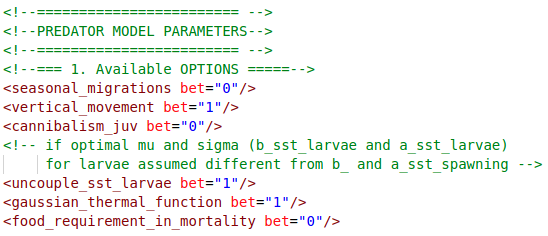
\includegraphics[width=0.7\textwidth]{chapter3/figs/options_available.png}
%   }
%   \caption{On this example of the bigeye model configuration the seasonal spawning migrations, cannibalism function and the use of food requirement index influencing mortality rates spatially, are switched off. The correction of velocities by the time spent in each pelagic layer as well as the Gaussian thermal function in the species accessibility function are used in most SEAPODYM configurations.}
%   \label{fig:options_parfile}
% \end{figure}

\subsubsection{Aggregation zones}
\label{sec:aggregation}

The aggregation zones can be defined for regional extractions of biomass and catch statistics, mainly for comparison with Multifan-CL model stock assessment. The extractions over EEZ (Exclusive Economic Zones) polygons can also be useful in model analyses and validations. Table~\ref{tab:configuration_aggregation_zones_1} describes the configuration parameters setting up the regional structure, both for rectangular regions and EEZs. If {\ttfamily nb\_region} is non-zero then the SEAPODYM output file SumQArea.txt will contain the biomass  by life stage and catch statistics by fishery, extracted over defined regions (see more details on the SumQArea.txt file in section~\ref{sec:SumQArea}). Otherwise, this file will be empty. Likewise, if the number of EEZ areas {\ttfamily nb\_EEZ} is non-zero and the EEZ mask file is provided (Table~\ref{tab:configuration_aggregation_zones_1}), then the output files, one by EEZ, called SumEEZ\_eezname.txt will be written in the output directory (see section~\ref{sec:SumEEZ}). The mask file with EEZ polygons can be generated by the GMB software (Appendix~\ref{sec:GMB}).

The regional structure is usually set up to match the Multifan-CL regions. The attributes named {\ttfamily areaN} with $\texttt{N}=0,\dots,\left(\texttt{nb\_region}-1\right)$ contain the corners of rectangular regions (see example on panel (a), Figure~\ref{fig:aggregation_zones}). The parameters {\ttfamily nb\_region\_sp\_B} and {\ttfamily area\_sp\_B} allow the selection of the subset of defined regions. It can be practical to compare the biomass predictions only in areas observed through fisheries data, which define estimations of a stock assessment model. If the configuration parameter {\ttfamily use\_mask\_catch} is set to $1$, then the SEAPODYM biomass will be extracted only from the grid cells with total catch (computed over the simulation time period) exceeding 1\% of the total catch over the domain.   

The extractions over EEZ areas can be done based on the EEZ mask file, which has the same format as the landmask file (see section~\ref{sec:land_mask}), with the mask being a matrix of dimensions of model spatial resolution $n_x \times n_y$ containing negative values in the grid cells inside EEZ or high seas areas. These values should be entered as EEZ IDs to activate EEZ extractions. Note, the EEZ mask file must contain all values set up in {\ttfamily EEZ} node. Example of EEZ extraction set-up is shown on panel (b) of Figure~\ref{fig:aggregation_zones}.

\begin{table}[H]
\caption{Set-up parameters for the regional extractions over rectangular or EEZ areas.}
\begin{tabular}{p{4cm}p{11.75cm}}
    \hline
    {\bfseries Parameters} & {\bfseries Description}\\ \hline\hline
    \multicolumn{2}{c}{\textit{Stock assessment regions}}\\
    \hline
    {\ttfamily nb\_region} & Number of rectangular regions. \\\hline
    {\ttfamily use\_mask\_catch} & A flag to activate (1) or deactivate (0) the use of catch mask in biomass extractions. If ``$1$'', then only the cells with $C^{tot}_{i,j}>1\%$ of $C^{tot}$ will be used in biomass extraction. \\\hline
    {\ttfamily areaN} & The IDs and coordinates of $0,\dots,\left(\texttt{nb\_region}-1\right)$ rectangular region.\\
	{\ttfamily nb\_region\_sp\_B} & The number of regions selected for modelled species. In single species simulations {\ttfamily nb\_region\_sp\_B} is usually the same as {\ttfamily nb\_region}. \\ 
	\hline
	{\ttfamily area\_sp\_B} & Vector of indices of considered regions with values from ``$1$'' to {\ttfamily nb\_region}.  \\ 
	\hline
	\multicolumn{2}{c}{\textit{Exclusive Economic Zones}}\\
	\hline
	{\ttfamily nb\_EEZ} & Number of EEZ areas to be used for biomass extractions. \\ 
	\hline	
	{\ttfamily str\_file\_maskEEZ} & EEZ mask file with negative values in grid cells inside EEZs or high seas area. \\ 
	\hline
	{\ttfamily eezN} & Names and IDs of $0,\dots,\left(\texttt{nb\_eez}-1\right)$ EEZ areas provided in the {\ttfamily str\_file\_maskEEZ} file.\\\hline
\end{tabular}
\label{tab:configuration_aggregation_zones_1}
\end{table}


\newpage
\begin{figure}[H]
   \centering
    \vbox{
    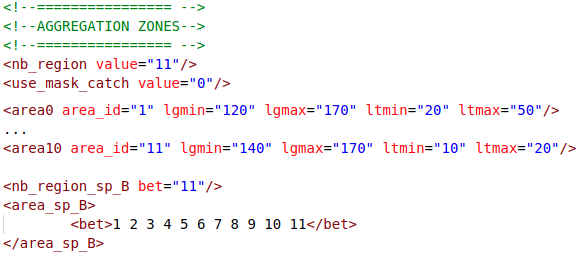
\includegraphics[width=0.75\textwidth]{chapter3/figs/aggregation_zones_1}\\
    (a)\\
     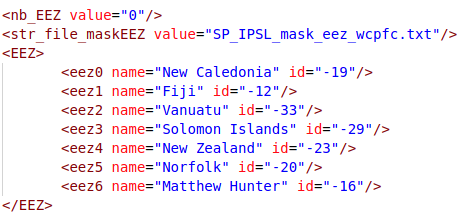
\includegraphics[width=0.6\textwidth]{chapter3/figs/aggregation_zones_2}\\
    (b)\\
   }
   \caption{
   Configuration of aggregation zones in the bigeye model parfile. (a): Rectangular regions for comparisons with stock assessment models. (b): EEZ areas configuration. Note that by convention the EEZ IDs are always negative numbers.}
   \label{fig:aggregation_zones}
 \end{figure}


\section{Running modes}\label{sec:running-modes}

The SEAPODYM computer application is not limited to a simulation mode executing numerical resolution of model~\ref{eq:model-1}. It is the modelling framework that allows running simulations, estimating model parameters, generating and estimating parameters of habitat indices alone, running tag simulator or a virgin population model with observed density used to inform model parameters. There are also additional functionalities necessary in the development of quantitative models. They include sensitivity analyses, Hessian matrix evaluation and likelihood profiling. This section explains how to set up available running modes, to run the application in these modes, and what to expect during the runtime. 

\subsection{Simulation}\label{sec:simulation-run} 
The basics of a simulation run are explained in section~\ref{sec:inputdir}. At the end of the simulation run, the parfile named {\ttfamily newparfile.xml} is written in the run directory and the restart file with final distributions of modelled density at age (section~\ref{sec:dym-files_outputs}) is saved in the output directory. Note that during a simulation run all parameter values are fixed regardless of the declaration in the {\ttfamily use} attribute. The exception occurs if the value of a control parameter ({\ttfamily use="true"}) is outside its boundaries, in which case the parameter value is reset to the value close to the nearest boundary before the numerical model resolution. The warning appears in the screen log. This behaviour is coded primarily for the optimization run, but is conserved for all other types of run.

\subsection{Habitats}\label{sec:habitat-run}
This is another type of a simulation run designed to compute habitats only, either spawning or feeding for a given age(s). It is executed with a standalone model build as a result of  compilation of SEAPODYM source code with the {\ttfamily Makefile\_habitats}, providing the executable binary file called {\ttfamily seapodym\_habitats}. This binary expects the following configuration parameters to be present in the parfile:

\vspace{0.35cm}
{\ttfamily
<habitat\_run\_type="flag" nb\_ages="value"/>\\
\indent <habitat\_run\_ages> index1 index2 $\dots$ indexN </habitat\_run\_ages>\\
}

\noindent where the {\ttfamily flag} ``0'' activates the spawning habitat simulation and flag=1 activates the feeding habitat simulation. Since the spawning habitat does not depend on age, only this flag is taken into account. In addition, the following DYM file accessible from the run directory, in sub-folder ``habitats'' should be provided for the spawning habitat simulation:

\vspace{0.2cm}
{\ttfamily 
\indent <spname>\_spawning\_habitat\_input.dym\\
} 

\noindent The time series of spatial distributions in this DYM file are assumed to contain habitat observations, which will be used by the MLE method in the estimation of spawning habitat parameters. The temporal dimension and the time interval of the time series in the input DYM file is required to match the run configuration. Note, if the purpose of this run is simulation only, the input DYM file does not affect the model outputs. In this case, a ``false'' input, for example, a softlink to any DYM file with a SEAPODYM variable, can be used.  

For the feeding habitat simulation, set the {\ttfamily habitat\_run\_type} to ``1'' and choose the {\ttfamily value} to indicate the number of age classes for which the feeding habitats should be  simulated. The attribute {\ttfamily habitat\_run\_ages} allows the age classes to be selected, with the indices corresponding to those of the age classes defined in the parfile (note, count starts at 0). Likewise, for the feeding habitat simulations, the input DYM files need to be provided as well in the run directory, sub-folder ``habitats''. However, in the case of an age-dependent feeding habitat, the software will require one file per age class:

\vspace{0.2cm}
{\ttfamily 
\indent <spname>\_feeding\_habitat\_input\_age1.dym\\
\indent <spname>\_feeding\_habitat\_input\_age2.dym\\
\indent ...\\
\indent <spname>\_feeding\_habitat\_input\_ageN.dym\\
} 

\noindent It is the user's responsibility to make sure that the input files contain the data for selected age classes. Then the habitat simulation is run by the command:\\

\vspace{0.35cm}
{\ttfamily
  seapodym\_habitats -s parfile.xml\\
}
\vspace{0.2cm}


\noindent and the estimation of habitat parameters is launched by the command:\\

\vspace{0.35cm}
{\ttfamily
  seapodym\_habitats parfile.xml\\
}
\vspace{0.2cm}

\noindent See more details on the optimization mode below and in Chapter~\ref{ch:parametrisation}.

\subsection{Density} \label{sec:density-run}
Just as for the habitat simulation runs, this running mode can be executed by the binary file compiled with a different Makefile, called {\ttfamily Makefile\_densities} and the input data is required for estimating the parameters based on fitting to the observed (or modelled) density fields. The input file should contain the aggregated over age dimension density, called {\ttfamily spname\_density\_input.dym}. The simulation run starts by the following command:

\vspace{0.35cm}
{\ttfamily
  seapodym\_densities -s parfile.xml\\
}

\noindent while the parameter estimation run is activated without any option.

\subsection{Optimization}\label{sec:optimization-run}
As pointed out above, the SEAPODYM application launched without any option will start the run with optimization. A prompt will appear waiting for a confirmation that the intention was to run the optimization method. However, the user is strongly advised to read Chapter~\ref{ch:parametrisation} prior to the use of this running mode. Several caveats related to the use of memory can lead to the execution problems in the configurations with high resolutions and large model dimensions, in which case the optimization run may require an increase in volume for memory allocation. 

If executed successfully, at the end of the optimization experiment the program runs a simulation run with estimated parameters. The {\ttfamily{newparfile.xml}}, written at the end of this simulation will contain the updated values of the total likelihood function and model parameters. More details on the execution of optimization runs can be found in Chapter~\ref{ch:parametrisation}, section~\ref{sec:fmin}.

\subsection{Likelihood profiling}\label{sec:profiling-run}

This running mode executes the likelihood profiling with respect to two selected parameters. This mode is activated with the command:
\vspace{0.35cm}

{\ttfamily
  seapodym -p parfile.xml
}
\vspace{0.35cm}
\noindent with the following (example) configuration parameters to be added in the XML parfile:

\vspace{0.5cm}
{\ttfamily
	<hyperspace$\_$projection>
	
\hspace{0.5cm} <variables nb="2"/>
        
\hspace{0.5cm} <spname name="a\_sst\_spawning" nsteps="5" />
        
\hspace{0.5cm} <spname name="nb\_recruitment" nsteps="5" />
        
	</hyperspace$\_$projection>
}
\vspace{0.5cm}

\noindent In this example, parameters {\ttfamily a\_sst\_spawnin} and {\ttfamily nb\_recruitment} were chosen from the list of control parameters. As a result, the program will split the parameter plane bounded by values specified by {\bfseries min} and {\bfseries max} attributes (section \ref{sec:mle_parameters}) into 25 intervals and run simulations to evaluate the likelihood within each interval. During the run, SEAPODYM writes an ASCII file in a matrix format with a header, called  {\ttfamily hyperproj.out}, of the following format:

\vspace{0.5cm}
{\ttfamily
\noindent 
\indent v1.name v2.name\\
\indent nbp1 nbp2\\
\indent v1.val1 v1.val2 ... v1.val.nbp1\\
\indent v2.val1 v2.val2 ... v2.val.nbp2\\
\\
\indent <nbp1 x nbp2 matrix with likelihood values>
}
\vspace{0.5cm}

\noindent where {\ttfamily v1} and {\ttfamily v2} denote two control variables (model parameters) and {\ttfamily nbp1} and {\ttfamily nbp2} are the number of points between (min, max) boundaries of each parameter.  

\subsection{Hessian computation}\label{sec:hessian-run}

The Hessian is computed in order to evaluate the uncertainty of estimated model parameters. This mode is practical only after the convergence of optimization to the set of MLE parameters. For the sake of time saving, the computation of the Hessian is not done automatically after each optimization run, and is launched manually, once the minimum is attained, and written to the {\ttfamily newparfile.xml}

\vspace{0.35cm}

{\ttfamily
  seapodym -h newparfile.xml
}
\vspace{0.35cm}

\noindent The ASCII file generated by this run, called {\ttfamily Hessian.out}, structured as follows: 

\vspace{0.35cm}
{\ttfamily
\noindent 
\indent nvar\\
\indent names values derivatives\\
\indent det(H)\\
\indent eigenvalues\\
\indent variance-covariance matrix\\
}

\noindent with the tags above corresponding to the number of variable parameters, their names, values and likelihood gradient components with respect to each variable, Hessian determinant, eigenvalues and variance-covariance matrix respectively.

\subsection{Sensitivity analyses}\label{sec:sensitivity-run}
Two types of sensitivity analyses are implemented in the SEAPODYM modelling framework. These are: i) local sensitivity analysis based on gradient information, computing either the likelihood function gradient or the gradient of a quadratic function including model predictions only; ii) global sensitivity analysis including evaluation of the first-order sensitivity indices and the total-effect sensitivity indices (see Chapter~\ref{ch:parametrisation}, section~\ref{sec:SA} for more details). These analyses can be activated simply by running the {\ttfamily seapodym} application with options {\ttfamily -sa=FLAG}, where {\ttfamily FLAG} takes values between 0 and 4 to execute one of the following runs: 

\begin{itemize}
\item[0:] local sensitivity analysis based on evaluation of the gradient of model prediction function; each run generates a single vector of local sensitivity measures, with number of elements being the number of parameters;
\item[1:] local sensitivity analysis based on evaluation of the gradient of the likelihood function, thus including both predictions and observations; same as for flag ``0'' - sensitivity measures are evaluated for a given parameter value;
\item[3:] a series of jitter simulation runs as a part of One-At-a-Time type of global sensitivity analysis; each run will evaluate the function value multiple times by varying only one parameter while keeping others fixed;
\item[4:] a simulation run as a part of All-At-a-Time type of global sensitivity analysis; the outcome of this simulation is simply the output function (usually selected likelihood term) value.
\end{itemize}

\section{SEAPODYM Outputs}
\label{sec:seapodym-outputs}
A simulation run produces multiple outputs: a series of text ASCII files aggregating predicted variables by region (see~\ref{sec:aggregation}) or all domain, and binary DYM files with 3D (2D space and time/age) variables. This section provides information on the contents of these outputs. The formats of ASCII and DYM files are described in Appendix~\ref{annex:file-formats}, sections~\ref{annex:sumdym}--\ref{annex:dymfile}. The GUI tool SeapodymView that can be used for manipulation and visualisation of SEAPODYM input and output files, both binary DYM files and ASCII files with fisheries data, is presented in Appendix~\ref{annex:toolbox}.  

\subsection{Setting the outputs directory}

The path to the output directory is provided in the parfile as follows:

\begin{center}
{\ttfamily 
<strdir\_output value = "output/">}
\end{center}

\noindent where the directory called {\ttfamily output} is the default location of model outputs, which is created (if not existing) in the run directory. The full path to an existing directory can also be specified. Note, if the specified directory does not exist, the program will write outputs to the default location.  

 
\subsection{Outputs in DYM files} \label{sec:dym-outputs}

The two-dimensional variables are written in SEAPODYM in binary DYM format. Table~\ref{tab:dym-outputs} provides a complete list of files, units and writing rules.


\begin{longtable}{p{3.25cm}p{8cm}p{2cm}p{1.25cm}}
\caption{All DYM files generated by a simulation, either by default or at user's request.\label{tab:dym-outputs}}\\
\textbf{Name}	& \textbf{Description} & \textbf{Units} & \textbf{Status} \\\hline 
\endfirsthead
\multicolumn{4}{@{}l}{Table continued}\\\hline
\textbf{Name}	& \textbf{Description} & \textbf{Units} & \textbf{Status} \\\hline 
\endhead % all the lines above this will be repeated on every page
\hline
%\multicolumn{3}{r@{}}{continued \ldots}\\
\endfoot
\hline
\endlastfoot
 \multicolumn{4}{c}{\texttt{ Population density}} \\
    \hline  
 {\ttfamily spname\_larve} & density of the larvae in number of individuals (Nb) per square kilometer & $\text{Nb}\cdot \text{km}^{-2}$ & default \\ 
 {\ttfamily spname$\_$juvnl} & density of juveniles (sum of density from age $1$ to the last specified age class in juvenile stage) & $\text{Nb}\cdot \text{km}^{-2}$ & default \\ 
{\ttfamily spname$\_$recru} & density at age of recruitment to the exploited population & $\text{Nb}\cdot \text{km}^{-2}$& default\\
{\ttfamily spname$\_$young} & biomass density of young (sum of density across all age classes within young life stage) in metric tonnes (mt) per square kilometer & $\text{mt}\cdot \text{km}^{-2}$& default\\
{\ttfamily spname$\_$adult} & biomass density of adults (sum of density across the adult life stage)& $\text{mt}\cdot \text{km}^{-2}$ & default\\
{\ttfamily spname$\_$totbm} & total biomass density (sum of young and adult life stage) & $\text{mt}\cdot \text{km}^{-2}$ & default\\
{\ttfamily spname$\_$ageN} & density of age class N. There should be a line in the parfile {\ttfamily write\_all\_cohorts\_dym value="1"}& $\text{Nb}\cdot \text{km}^{-2}$& on demand\\   
 \hline   
 \multicolumn{4}{c}{\texttt{ Fisheries data}} \\ 
 \hline  
{\ttfamily spname\_Cobs} &total observed catch in model units & mt or Nb& default\\
{\ttfamily spname\_Cobs\_f}& observed catch by fishery 'f'. There should be a line in the parfile {\ttfamily write\_all\_fisheries\_dym value="1"} & mt or Nb& on demand\\    
{\ttfamily spname\_Cpred}& total predicted catch in model units  &mt or Nb & default\\  
{\ttfamily spname\_Cpred\_f}& predicted catch by fishery 'f'. There should be a line in the parfile {\ttfamily write\_all\_fisheries\_dym value="1"} &mt or Nb& on demand\\
 \hline
 \multicolumn{4}{c}{\texttt{ Movement rates}} \\     
 \hline
{\ttfamily spname\_Vtot\_x}& zonal velocity of the oldest fish (A+ class) in nautical miles (nmi) per month (mo), including both passive (zonal current velocity) and active (taxis) components. Positive to the east. & $\text{nmi}\cdot\text{mo}^{-1}$ &  default\\
{\ttfamily spname\_Vtot\_y}& meridional velocity of the oldest fish (A+ class) including both passive (meridional current velocity) and active (taxis) components. Positive to the north & $\text{nmi}\cdot\text{mo}^{-1}$& default\\
{\ttfamily spname$\_$speed}& speed of fish in A+ class & $\text{nmi}\cdot\text{mo}^{-1}$   & default\\
{\ttfamily spname$\_$diffusion} & diffusion rate of the oldest fish  & $\text{nmi}^{2}\cdot\text{mo}^{-1}$ & default\\
 \hline
 \multicolumn{4}{c}{\texttt{ Habitat indices}} \\     
 \hline
{\ttfamily spname$\_$Ha\_first} {\ttfamily \mbox{   }\_maturity}& feeding habitat index of fish in the first 50\% maturity age class in adult life stage& &default\\   
{\ttfamily spname$\_$Ha\_oldest}& feeding habitat index of fish in A+ age class& &default\\   
 \hline
 \multicolumn{4}{c}{\texttt{ Restart file}} \\     
 \hline 
 {\ttfamily spname$\_$cohorts} {\ttfamily \mbox{   }yyyy\_mm}& density of all age classes at a given time step (written at the end of a simulation)& $\text{Nb}\cdot \text{km}^{-2}$ & default\\
 \hline
\end{longtable} 


Each file contains a header and the time series of the two-dimensional field (see Appendix~\ref{annex:dymfile} for details on file format and structure). Hence, the dimensions of the variable written in the DYM file is Zlevel~$\times$~Nlat~$\times$~Nlong
where Nlat, Nlong, Zlevel are the latitudinal and longitudinal dimensions and the number of time steps. 

\subsubsection{Population density by life stage} 
For classification of life stages in SEAPODYM see Table~\ref{tab:life_stages}. The population density for larvae and juveniles is computed as the sum over all age classes within each life stage:
\begin{equation*}
    N(t,x,y) = \sum_{a} N(a,t,x,y) 
\end{equation*}
with $N(a,t,x,y)$ the density of fish of age $a$ in $\text{Nb/km}^{2}$ (model units of the state variables), at the coordinates ($x$,$y$) and at time $t$. Age $a$ is either equal to $0$ for larvae, or from $1$ to the last age in juvenile life stage. \\ 

For young and adults the biomass density is multiplied by the mean weight, $w(a)$, of each age class and so the unit becomes $\text{mt/km}^{2}$. The mean weights can be found in the parfile (see Table~\ref{fig:age_structure_parfile}). So, for the biomass density we have:  
\begin{equation*}
    N(t,x,y) = \sum_{a} w(a)N(a,t,x,y) 
\end{equation*}
\noindent with $a\in\left[\text{age\_autonomous to age\_maturity-1} \right]$ for young, and $a \in\left[\text{age\_maturity to $A^{+}$}\right]$ for adults. Note, the numerical solution of model~\ref{eq:model-1}, that is spatial distributions $N(a,t,x,y)$, corresponds to the end of the time step (see Chapter~\ref{ch:numerics}, sections~\ref{sec:d-time} and \ref{sec:two-steps-splitting-method}). \\ 

\subsubsection{Movement rates} 

The velocity vector components (both passive and active) and the diffusion rate varying with habitat index are saved only for the last age class, A+. The speed of population density at age A+ is computed from the advection velocity field $\mathbf{v}(t,x,y)=(u(t,x,y),v(t,x,y)$ as:

\begin{equation*}
    V(x,y,t) = \sqrt{u(t,x,y)^2+v(t,x,y)^2}
\end{equation*}

\noindent where $u\in\mathbb{R}$, $v\in\mathbb{R}$, V $\in\mathbb{R^{+}}$, and D$\in\mathbb{R^{+}}$.

\subsubsection{Predicted and observed catches}

The predicted catches are computed in the model and written in units defined in the parfile (see section~\ref{sec:config-fisheries}), hence either in metric tonnes or in number of fish. Note, currently the model application does not support different units by fishery. 
  
\subsubsection{Habitat indices}  
Only two habitat files are saved: one at the age of first 50\% maturity, and another for the oldest adults. In order to output habitats for all or selected age classes, use the {\ttfamily seapodym\_habitats} application (see section~\ref{sec:habitat-run}).

\subsubsection{Restart}\label{restart-dym}
The date {\ttfamily yyyy-mm} corresponding to the last date of a simulation run is stored only in the file name. Since age dimension is used instead of time in the DYM file, the Zlevel vector contains age information. This restart file can then be used as the {\ttfamily init file}(~\ref{sec:init-dym}). It is the user's responsibility to manage the time stamp of the state vector. 

\subsection{ASCII output files}

\underline{Here is a list of the ASCII files generated by a simulation:}
\begin{itemize}
    \item[-] {\ttfamily SumDym.txt} : for every time step of a simulation, total primary production, total biomass of micronekton groups, total biomass of population by life stage, fishing effort by fishery, observed and predicted catch by fishery.  
    \item[-] {\ttfamily SumQArea.txt}: for every time step of a simulation, total population biomass by life stage and by region.
    \item[-] {\ttfamily SumEEZ\_ID.txt}: for every time step of a simulation, total population biomass by life stage and by EEZ.    
      \item[-] {\ttfamily spname\_MeanVar.txt}: spatial mean of mortality, advection and diffusion rates by age class.
       \item[-] {\ttfamily spname\_Spatial\_Corr.txt}: spatial correlation between predicted and observed catch.
    \item[-] {\ttfamily spname\_LF\_obs.txt}: observed length frequency by region aggregated over the whole time series in 4 quarters and in total.
    \item[-] {\ttfamily spname\_LF\_Q\_fishery.txt}: length frequency of catch by fishery and by quarter.
    \item[-] {\ttfamily spname\_LF\_Q\_sum.txt}: catch by age, by region and by fishery; quarterly sums for overall time period.
\end{itemize}

The following sections describe the contents of each file, while the file structure can be found in Appendix~\ref{annex:text-files}.

\subsubsection{{\ttfamily SumDym.txt}}

This file gives the time evolution of model variables aggregated over the entire domain. In other words, if we denote $\phi(x,y,t)$ the variable of interest, the file contains $\sum\limits_{x,y}\phi(x,y,t)$. 

\begin{table}[H]
\caption{Configuration parameters and variables written in the {\ttfamily SumDym.txt} file.}
\raggedleft
\begin{tabular}{p{4cm}p{11.75cm}}
    \hline
    {\bfseries Parameters} & {\bfseries Description}\\ \hline\hline
    {\ttfamily date} & The date of the time step given as {\ttfamily yyyy-m-d}) \\ \hline
    {\ttfamily tstep} & The time step \\
    \hline
    {\bfseries Variables} & {\bfseries Description}\\ \hline\hline
    {\ttfamily P in C-C}  & The total primary production, in mmol~C$\cdot\text{m}^{-2} \cdot\text{day}^{-1}$, in the regions bounded by the latitudinal coordinates $C-C$. There are three regions: 10N--45N,10S--10N  and 35S--10S \\\hline
    {\ttfamily P total}  & The total primary production over the area within $C-C$ coordinates, in  mmol~C$\cdot\text{m}^{-2} \cdot\text{day}^{-1}$.\\\hline
    {\ttfamily F$\_$xxx}  & Total biomass in mt of xxx-pelagic functional group of micronekton (among meso, hmeso, epi, bathy, mbath, hmbathy). \\ \hline
    {\ttfamily B life\_stage} {\ttfamily  spname}  & Total population biomass in mt by life stage (larvae, juvenile, recruitment, young, adult)\\ \hline
    {\ttfamily B total} {\ttfamily spname}  & Total population biomass in metric tonnes (mt).\\ \hline
    {\ttfamily effort} {\ttfamily fisheryID} & Effort by fishery, in units provided for fishery with a short name {\ttfamily fisheryID}. \\ \hline
    {\ttfamily obs C\_spname} {\ttfamily \_fisheryID} & Total observed catch by fishery in mt or Nb\\ \hline
    {\ttfamily pred C\_spname} {\ttfamily \_fisheryID} & Total predicted catch by fishery in mt or Nb\\ \hline
    {\ttfamily obs CPUE\_spname} {\ttfamily \_fisheryID} & The observed Catch Per Unit Effort by fishery, in units depending on units of catch and effort\\ \hline
    {\ttfamily pred CPUE\_spname} {\ttfamily \_fisheryID} & The predicted Catch Per Unit Effort by fishery, in units depending on units of catch and effort\\
    \hline
\end{tabular}
\label{tab:variables_sumdym}
\end{table}

\subsubsection{{\ttfamily SumQArea.txt}}
\label{sec:SumQArea}
This file stores the predicted population abundance (either as total number of fish or as total biomass) aggregated over the rectangular regions defined in the parfile (see section~\ref{sec:aggregation}). The population abundance is calculated for different life stages (for classification of life stages in SEAPODYM see Table~\ref{tab:life_stages}). Providing the age at recruitment to the exploited stock and the regional structure as defined in a given stock assessment model, these aggregated outputs can be used for comparisons with the stock assessment model outputs. The variables in the file are detailed in Table~\ref{tab:variables-sumqarea}. See the structure of this file in Appendix~\ref{annex:sumqarea}. \\
 
\begin{table}[H]
\caption{Configuration parameters and model variables written in the {\ttfamily SumQArea.txt} file}
\raggedleft
\begin{tabular}{p{4cm}p{11.75cm}}
    {\bfseries Parameters} &  {\bfseries Description}\\ \hline \hline
    {\ttfamily regional coordinates} & The lon-lat coordinates of the corners of rectangular regions defined in the {\ttfamily area} node in the parfile. \\ 
    \hline
    {\ttfamily life stage} & The indices of the age classes in each life stage\\
    \hline
     {\ttfamily date} & Date written as {\ttfamily year}, {\ttfamily month} and {\ttfamily day} columns \\\hline 
    {\bfseries Variables} &  {\bfseries Description}\\ \hline \hline
    {\ttfamily spname N} {\ttfamily life\_stage} {\ttfamily region r}  & Total number of fish by life stage (from larval stage to recruits) in region $r$ \\ 
    \hline
    {\ttfamily Total N} {\ttfamily life stage}  & Total number of fish from larval stage to recruits over all regions\\ \hline
    {\ttfamily spname B} {\ttfamily life\_stage} {\ttfamily region r}  & Total biomass of fish by life stage (for immature and mature adults) in region $r$ \\ 
    \hline
    {\ttfamily spname B tot.} {\ttfamily region r}  & Total biomass of fish at adult stage (immature and mature combined) in region $r$.\\ 
    \hline
    {\ttfamily Total B}  & Total biomass of adult fish over all regions\\
    \hline
\end{tabular}
\label{tab:variables-sumqarea}
\end{table}

\subsubsection{{\ttfamily SumEEZ.txt}}\label{sec:SumEEZ}

These files have exactly the same variables as SumQArea.txt, but the EEZ area is used for biomass aggregation instead of rectangular regions. 

\subsubsection{{\ttfamily MeanVar.txt}}
\label{sec:MeanVar}
This file, used for diagnostics, contains the spatial mean of different two-dimensional fields computed but not written in DYM files. The contents of the file are listed in Table~\ref{table:variables_MeanVar}. Each variable is provided by age class, from $0$ to the last $A^{+}$ age class.\\

\begin{center}
\begin{table}[H]
\caption{Configuration parameters and variables written in the {\ttfamily spname\_MeanVar.txt} file. }
\raggedleft
\begin{tabular}{p{4cm}p{11.75cm}}
    {\bfseries Parameters} & {\bfseries Description}\\ \hline \hline
    {\bfseries date} & Written in {\ttfamily year, month, day} columns\\ \hline
    {\bfseries Variables} & {\bfseries Description}\\ \hline \hline
    {\ttfamily mortality-at-age p}  & Mean mortality rate ({$\text{mo}^{-1}$}) of the species {\ttfamily spname} at age $a_p$. \\ \hline
    {\ttfamily speed p}  & Mean speed (nmi$\cdot\text{mo}^{-1}$) of the species {\ttfamily spname} at age $a_p$.\\ \hline
   {\ttfamily diffusion p}  &  Mean diffusion rate (nmi$^2\cdot\text{mo}^{-1}$) of the species {\ttfamily spname} at age $a_p$. \\ \hline
   {\ttfamily temperature p}  & Mean water temperature ($^\circ$C) weighted by the population density at age $a_p$. \\
    \hline
\end{tabular}
\label{table:variables_MeanVar}
\end{table}
\end{center}

\subsubsection{{\ttfamily Spatial\_Corr.txt}}
The spatial correlations between the observed and predicted catches as well as Student test probability values are computed at each time step for all fisheries and written in file {\ttfamily Spatial\_Corr.txt} (Table~\ref{tab:variablesCORR}). \\

\begin{center}
\begin{table}[H]
\caption{Configuration parameters and variables written in the {\ttfamily Spatial\_Corr.txt} file.}
\begin{tabular}{p{4cm}p{11.75cm}}
    \hline
    {\bfseries Variables} & {\bfseries Description}\\ \hline\hline
    {\ttfamily n}  & Number of values used to compute correlation. \\ \hline
    {\ttfamily r\_fishery spname}  & Correlation between observed and predicted catches by fishery. \\ \hline
    {\ttfamily prob}  & Student estimation. \\ \hline
    {\ttfamily CPUE$\_$r\_fishery spname}  & Correlation between the observed and the predicted CPUE by fishery.\\\hline
    {\ttfamily prob}  & Student estimation. \\
    \hline
\end{tabular}
\label{tab:variablesCORR}
\end{table}
\end{center}

\subsubsection{{\ttfamily spname\_LF\_obs.txt}}
This file gives both the observed catch-at-age and the sum of catch-at-age per fishery, region and quarter (Table~\ref{tab:LFobs}). 

\begin{center}
\begin{table}[H]
\caption{Configuration parameters and variables written in the {\ttfamily spname\_LF\_obs.txt} file.}
\raggedleft
\begin{tabular}{p{4cm}p{11.75cm}}
    \hline
    {\bfseries Parameters} & {\bfseries Description}\\ \hline\hline 
    {\ttfamily Length} & Mean lengths in age classes, in cm. \\\hline
    {\bfseries Variables} & {\bfseries Description}\\ \hline\hline 
    {\ttfamily f\_spname\_region\_r}  & Observed catch-at-age by fishery $f$ and region $r$.\\ \hline
    {\ttfamily sum\_f\_spname}  & Total observed catch-at-age by fishery $f$ over all regions.\\ \hline
    {\ttfamily sum\_spname\_region\_r}  & Total  observed catch-at-age for all fisheries in region $r$.\\
    \hline
\end{tabular}
\label{tab:LFobs}
\end{table}
\end{center}


\subsubsection{{\ttfamily spname$\_$LF$\_$Q$\_$fishery.txt}}
\label{file:LFQfishery}
This file contains the predicted length frequencies aggregated over model age classes (catch-at-age) per quarter, per fishery and per region (Table~\ref{tab:LFQfishery}). It has the same tabular format as the input LF data file (see Appendix sections~\ref{sec:LF-datafile} and \ref{sec:lfqfishery}). \\

\begin{center}
\begin{table}[H]
\caption{Configuration parameters and variables written in the {\ttfamily spname$\_$LF$\_$Q$\_$fishery.txt} file}
\raggedleft
\begin{tabular}{p{3cm}p{12.5cm}}
    \hline
    {\bfseries Parameters} & {\bfseries Description}\\ \hline\hline 
    {\ttfamily Fisheries} & Fishery ID \\\hline
    {\ttfamily Regions} & Region ID \\\hline
    {\ttfamily date} & Date written in the columns Year, Quarter and Month \\\hline
    {\bfseries Variables} & {\bfseries Description}\\ \hline\hline 
    {\ttfamily LF[p]}  & Predicted catch-at-age in number of fish of age $a_p$ caught by fishery in a given region\\
    \hline
\end{tabular}
\label{tab:LFQfishery}
\end{table}
\end{center}


\subsubsection{{\ttfamily spname$\_$LF$\_$Q$\_$sum.txt}}
\label{file:sumLFQfishery}
Together with the file {\ttfamily spname$\_$LF$\_$Q$\_$fishery.txt}, this file is mostly used for model validation, as it provides detailed information on the age distribution of catches by fishery, region and quarterly time intervals predicted by the model. Note, quarter is the time interval at which the LF data are collected. 

The row with the total catch-at-age data corresponding to the mean length $l$, for quarter $q$ of the column {\ttfamily fisheryID\_spname\_region\_r} is computed from the sum of the values written in the file {\ttfamily spname$\_$LF$\_$Q$\_$fishery.txt} for corresponding  date $D$, region $r$, fishery $f$ and quarter $q$:

\begin{equation*}
    \sum_{D\in\left[q_{i}\cap r\cap F\right]}\text{LF}\left[l\right]_{D}.
\end{equation*}

\begin{center}
\begin{table}[H]
\caption{Configuration parameters and variables written in the {\ttfamily spname$\_$LF$\_$Q$\_$sum.txt} file.}
\begin{tabular}{p{4cm}p{11.75cm}}
    \hline
    {\bfseries Parameters} & {\bfseries Description}\\ \hline\hline
    {\ttfamily length} & The mean length in cm of the age class. \\ \hline
    {\bfseries Variables} & {\bfseries Description}\\ \hline\hline
    {\ttfamily fisheryID} {\ttfamily \_spname}{\ttfamily \_region\_r} & Predicted catch-at-age by fishery in number of individuals (Nb) of age class with mean length $l$, in region $r$ during quarter $q$ \\ \hline
    {\ttfamily sum\_fisheryID} {\ttfamily \_spname} & Total predicted catch-at-age (Nb) by fishery over all regions during the quarter $q$ \\ \hline
    {\ttfamily sum\_spname} {\ttfamily \_region\_r}  & Total predicted catch-at-age (Nb) by all fisheries in region $r$ during quarter $q$\\
   \hline
\end{tabular}
\label{fig:sumQLFfishery}
\end{table}
\end{center}


\addcontentsline{toc}{section}{References}

%\reftitle{References}

\begin{thebibliography}{999}
%\bibitem[Author1(year)]{ref-journal}
%Author~1, T. The title of the cited article. {\em Journal Abbreviation} {\bf 2008}, {\em 10}, 142--149.
%% Reference 2
%\bibitem[Author2(year)]{ref-book1}
%Author~2, L. The title of the cited contribution. In {\em The Book Title}; Editor1, F., Editor2, A., Eds.; Publishing House: City, Country, 2007; pp. 32--58.
%% Reference 3
%\bibitem[Author3(year)]{ref-book2}
%Author 1, A.; Author 2, B. \textit{Book Title}, 3rd ed.; Publisher: Publisher Location, Country, 2008; pp. 154--196.
%% Reference 4
%\bibitem[Author4(year)]{ref-unpublish}
%Author 1, A.B.; Author 2, C. Title of Unpublished Work. \textit{Abbreviated Journal Name} stage of publication (under review; accepted; in~press).
%% Reference 5
%\bibitem[Author5(year)]{ref-communication}
%Author 1, A.B. (University, City, State, Country); Author 2, C. (Institute, City, State, Country). Personal communication, 2012.
%% Reference 6
%\bibitem[Author6(year)]{ref-proceeding}
%Author 1, A.B.; Author 2, C.D.; Author 3, E.F. Title of Presentation. In Title of the Collected Work (if available), Proceedings of the Name of the Conference, Location of Conference, Country, Date of Conference; Editor 1, Editor 2, Eds. (if available); Publisher: City, Country, Year (if available); Abstract Number (optional), Pagination (optional).

\bibitem[Autodif User's Manual, 2021]{Autodif} AUTODIF: A C ++ Array Language Extension with Automatic Differentiation For Use in Nonlinear Modeling and Statistics. \url{https://github.com/admb-project/admb/releases/download/admb-12.3/autodif-12.3.pdf} 

\bibitem [Bard, 1974] {Bard} 
Bard, Y. Nonlinear parameter estimation. Academic Press: New York, 1974.

\bibitem [Griewank and Corliss, 1991] {Griewank} 
Griewank, A.,  Corliss, G.F.  Automatic differentiation of algorithms: theory, implementation, and application. SIAM: Philadelphia, 1991.

\bibitem[Hampton and Fournier, 2001]{Hampton-Fournier}Hampton, J., and Fournier, D.A. 2001. A spatially disaggregated, length-based, age-structured population model of yellowfin tuna (Thunnus albacares) in the western and central Pacific Ocean. Mar. Freshw. Res. 52: 937–963. \url{https://doi.org/10.1071/MF01049}.

\bibitem[Fonteneau, 1996] {Fonteneau} 
Fonteneau, A. Interactions between tuna fisheries: a global review with specific examples from the Atlantic Ocean. In Status of Interactions of Pacific Tuna Fisheries in 1995. Proceedings of the Second FAO Expert Consultation on Interactions of Pacific Tuna Fisheries, Shimizu, Japan, 23–31 January 1995; R.S. Shomura, J. Majkowski, and R.F. Harman, Eds.; FAO Fisheries Technical Paper, 1996; No. 365.

%\bibitem [Langley et al., 2005]{MFCL-SKJ} Langley, A., Hampton, J., Ogura, M.  Stock assessment of skipjack tuna in the western and central Pacific Ocean. Western And Central Pacific Fisheries Commission, Scientific Committee,SA WP4). {\bf 2005}, http://wcpfc.org/sc1/pdf/SC1\_SA\_WP\_4.pdf 

\bibitem[Matear, 1995]{Matear} Matear, R. J. 1995. Parameter optimization and analysis of ecosystem models using simulated annealing: a case study at Station P.  {\em Journal of Marine Research.} {\bf 1995}, {\em 53}, 571--607. 

\bibitem[Otter Research Ltd, 1994]{Fournier} 
Otter Research Ltd. Autodif: a C++ array extension with automatic differentiation for use in nonlinear modeling and statistics. Otter Research Ltd: Nanaimo, Canada, 1994.

\bibitem[SPC Year Book, 2016] {Yearbook} Pacific Community (SPC). 2016. Tuna Fisheries Yearbook. Western and Central Pacific Fisheries Commission, Pohnpei, Federated States of Micronesia.

\bibitem[Pianosi et al., 2016]{Pianosi} 
Pianosi, F., Beven, K., Freer, J., Hall, J., Rougier, J., Stephenson, D., and Wagener, T. Sensitivity analysis of environmental models: A systematic review with practical workflow. Environ. {\em Modell. Softw.} {\bf 79}, 214–-232. \url{https://doi.org/10.1016/j.envsoft.2016.02.008}.

%continue formatting from here

\bibitem[Robinson and Lermusiaux, 2002]{Robinson} Robinson, A.R., Lermusiaux, P. F. J. 2002. Data assimilation for modeling and predicting coupled physical biological interactions in the sea. From \textit {The Sea}, Volume 12, edited by Allan R. Robinson, James J. McCarthy, and Brian J. Rothschild. John Wiley \& Sons, Inc., New York. 475-536.

\bibitem[Saltelli et al., 2008]{Saltelli} Saltelli, A., Ratto, M., Andres, T., Campolongo, F., Cariboni, J., Gatelli, D., et al. 2008. Global sensitivity analysis. The Primer. John Wiley and Sons.

\bibitem[Senina et al., 2008]{Senina08} Senina, I., Sibert, J., and Lehodey, P. 2008. Parameter estimation for basin-scale ecosystem-linked population models of large pelagic predators: Application to skipjack tuna. Prog. Oceanogr. 78: 319–335. doi:10.1016/j.pocean.2008.06.003.

%\bibitem[Senina et al., 2012]{Senina12} Senina, I., Royer, F., Lehodey, P., Hampton, J., Nicol, S., Ogura, M., et al. 2012. Integrating conventional and electronic tagging data into SEAPODYM. Pelagic Fish. Res. Prog. Univ. Hawaii Manoa Newslett. 16(1): 9–14.

\bibitem[Senina et al., 2020a]{Senina20a} Senina, I., Lehodey, P., Hampton, J. and J. Sibert. 2020a. Quantitative modelling of the spatial dynamics of South Pacific and Atlantic albacore tuna populations. \textit{Deep Sea Res. II}  175,  doi.org/10.1016/j.dsr2.2019.104667).  

\bibitem[Senina et al., 2020b]{Senina20b} Senina, I., Lehodey, P., Sibert, J. and J. Hampton. 2020b. Integrating tagging and fisheries data into a spatial population dynamics model to improve its predictive skills. \textit{Can. J. Aquat. Fish. Sci.} 77, 576–593.

\bibitem[Senina et al., 2020c]{Senina2020c} Senina, I., Lehodey, P., Nicol, S., Scutt Phillips, J., Hampton, J., 2020c. SEAPODYM: revisiting bigeye reference model with conventional tagging data. WCPFC-SC16-2020.

\bibitem[Sibert et al., 1999]{Sibert} Sibert, J.R., Hampton, J., Fournier, D.A., Bills, P.J. 1999. An advection-diffusion-reaction model for the estimation of fish movement parameters from tagging data, with application to skipjack tuna ({\it Katsuwonus pelamis}). \textit {Can. J. Fish. Aquat. Sci.} 56, 925-938. 

%\bibitem[Sibert and Hampton, 2003]{Sibert-Hampton} Sibert, J., Hampton, J. 2003. Mobility of tropical tunas and the implications for fishery management. \textit {Marine Policy} 27: 87-95.
%Procedings of the Second FAO Expert Consultation on Interactions of Pacific Ocean Tuna Fisheries, Shimizu, Japan, 23-31 January, 1995; FAO Fish. Tech. Pap. 365:402-418, Rome, 1996, 612pp. edited by R. S. Shomura, J. Majkowski, and R. F. Harman. 1996.

\bibitem[Taylor, 2001]{Taylor} Taylor, K.E. 2001. Summarizing multiple aspects of model performance in a single diagram. J. Geophys. Res. 106: 7183–7192. \url{https://doi.org/10.1029/2000JD900719}.

\bibitem[Vallino, 2000]{Vallino} Vallino, J.J. 2000. Improving marine ecisystem models: use of data assimilation and mesocosm experiments. \textit {Journal of Marine Research.} 58, 117-164.

\bibitem[Worley, 1991]{Worley} Worley, B. 1991. Experience with the forward and reverse mode of GRESS in contaminent transport modeling and other applications. In Griewank, A. and G.F. Corliss. Automatic differentiation of algorithms: theory, practice and application. SIAM, Philadelphia.

\end{thebibliography}
